\documentclass[11pt]{article}

\usepackage[letterpaper,margin=0.78in,headheight=15pt]{geometry}
\usepackage[T1]{fontenc}
\usepackage[utf8]{inputenc}
\usepackage{lmodern}
\usepackage{microtype}
\usepackage{amsmath,amssymb,mathtools}
\usepackage{booktabs,tabularx,array,longtable,multirow}
\usepackage{enumitem}
\usepackage{xcolor}
\usepackage{graphicx}
\usepackage{caption}
\usepackage{subcaption}
\usepackage{float}
\usepackage{tikz}
\usetikzlibrary{arrows.meta,positioning,calc,fit,backgrounds,decorations.pathreplacing,shapes.geometric,shapes.multipart}
\usepackage[most]{tcolorbox}
\usepackage{listings}
\usepackage{fancyhdr}
\usepackage{titlesec}
\usepackage{hyperref}
\usepackage[nameinlink,noabbrev]{cleveref}
\usepackage{xurl}

% Visual language follows the requested Gemma handout: dark ink, violet structure,
% teal mechanisms, restrained status boxes, and diagrams that carry argument rather
% than decoration.
\definecolor{ink}{HTML}{18222D}
\definecolor{slate}{HTML}{4D5B6A}
\definecolor{violet}{HTML}{6D5BD0}
\definecolor{violetdark}{HTML}{4E3DA8}
\definecolor{teal}{HTML}{0C7C86}
\definecolor{bluegray}{HTML}{EAF0F5}
\definecolor{lavender}{HTML}{F0EDFF}
\definecolor{mint}{HTML}{E9F7F4}
\definecolor{amber}{HTML}{A86500}
\definecolor{amberbg}{HTML}{FFF5DD}
\definecolor{redish}{HTML}{A43842}
\definecolor{redbg}{HTML}{FFF0F1}
\definecolor{greenish}{HTML}{277A55}
\definecolor{greenbg}{HTML}{EAF7F0}
\definecolor{sessionbg}{HTML}{FFF0EE}

\hypersetup{
  colorlinks=true,
  linkcolor=violetdark,
  citecolor=teal,
  urlcolor=teal,
  pdftitle={Shared Metadata Service and Persistent Catalog Cache: Design, Implementation, and Validation Review},
  pdfauthor={Prepared for Karl Burtram},
  pdfsubject={vscode-mssql PR 22836, metadata substrate design, implementation review, persistent cache, language service and STS2 integration}
}

\pagestyle{fancy}
\fancyhf{}
\lhead{vscode-mssql Metadata Substrate}
\rhead{Design, Implementation, and Validation Review}
\cfoot{\thepage}
\renewcommand{\headrulewidth}{0.4pt}

\titleformat{\section}{\Large\bfseries\color{ink}}{\thesection}{0.7em}{}
\titleformat{\subsection}{\large\bfseries\color{violetdark}}{\thesubsection}{0.65em}{}
\titleformat{\subsubsection}{\normalsize\bfseries\color{teal}}{\thesubsubsection}{0.55em}{}

\setlist[itemize]{topsep=3pt,itemsep=2pt,parsep=1pt,leftmargin=1.45em}
\setlist[enumerate]{topsep=3pt,itemsep=2pt,parsep=1pt,leftmargin=1.65em}
\setlength{\parindent}{0pt}
\setlength{\parskip}{5.5pt}
\setlength{\emergencystretch}{2em}
\raggedbottom

\newcommand{\code}[1]{\texttt{\detokenize{#1}}}
\newcommand{\impl}{\textcolor{greenish}{\textbf{Implemented}}}
\newcommand{\valid}{\textcolor{teal}{\textbf{Validated}}}
\newcommand{\future}{\textcolor{amber}{\textbf{Future contract}}}
\newcommand{\target}{\textcolor{violetdark}{\textbf{Target invariant}}}
\newcommand{\gap}{\textcolor{redish}{\textbf{Reviewed gap}}}
\newcommand{\reported}{\textcolor{slate}{\textbf{Reported evidence}}}
\newcommand{\na}{\textcolor{slate}{--}}
\newcommand{\yes}{\textcolor{greenish}{\checkmark}}
\newcommand{\partialmark}{\textcolor{amber}{$\triangle$}}
\newcommand{\no}{\textcolor{redish}{$\times$}}

\newtcolorbox{takeawaybox}[1][]{
  enhanced, breakable, colback=lavender, colframe=violet,
  boxrule=0.8pt, arc=2mm, left=2.5mm,right=2.5mm,top=1.8mm,bottom=1.8mm,
  fonttitle=\bfseries, title={Key takeaway}, #1
}
\newtcolorbox{statusbox}[1][]{
  enhanced, breakable, colback=bluegray, colframe=slate,
  boxrule=0.7pt, arc=2mm, left=2.5mm,right=2.5mm,top=1.8mm,bottom=1.8mm,
  fonttitle=\bfseries, title={Evidence status}, #1
}
\newtcolorbox{designbox}[1][]{
  enhanced, breakable, colback=mint, colframe=teal,
  boxrule=0.7pt, arc=2mm, left=2.5mm,right=2.5mm,top=1.8mm,bottom=1.8mm,
  fonttitle=\bfseries, title={Design invariant}, #1
}
\newtcolorbox{boundarybox}[1][]{
  enhanced, breakable, colback=amberbg, colframe=amber,
  boxrule=0.7pt, arc=2mm, left=2.5mm,right=2.5mm,top=1.8mm,bottom=1.8mm,
  fonttitle=\bfseries, title={Scope boundary}, #1
}
\newtcolorbox{warningbox}[1][]{
  enhanced, breakable, colback=redbg, colframe=redish,
  boxrule=0.7pt, arc=2mm, left=2.5mm,right=2.5mm,top=1.8mm,bottom=1.8mm,
  fonttitle=\bfseries, title={Validity warning}, #1
}
\newtcolorbox{reviewbox}[1][]{
  enhanced, breakable, colback=redbg, colframe=redish,
  boxrule=0.9pt, arc=2mm, left=2.7mm,right=2.7mm,top=2mm,bottom=2mm,
  fonttitle=\bfseries, title={Current-head review finding}, #1
}
\newtcolorbox{evidencebox}[1][]{
  enhanced, breakable, colback=bluegray, colframe=violetdark,
  boxrule=0.7pt, arc=2mm, left=2.5mm,right=2.5mm,top=1.8mm,bottom=1.8mm,
  fonttitle=\bfseries, title={Evidence boundary}, #1
}

\lstdefinestyle{code}{
  basicstyle=\ttfamily\small,
  backgroundcolor=\color{bluegray},
  frame=single,
  rulecolor=\color{slate!50},
  keywordstyle=\bfseries\color{violetdark},
  commentstyle=\itshape\color{slate},
  stringstyle=\color{teal},
  showstringspaces=false,
  breaklines=true,
  columns=fullflexible,
  xleftmargin=0.5em,
  xrightmargin=0.5em,
  aboveskip=6pt,
  belowskip=6pt
}
\lstset{style=code}

\tikzset{
  >=Latex,
  every node/.style={font=\small,text=ink},
  comp/.style={draw=slate!65,rounded corners=2.5pt,fill=bluegray,align=center,inner sep=4pt,minimum height=10mm},
  store/.style={comp,fill=lavender,draw=violet!75},
  model/.style={comp,fill=mint,draw=teal!75},
  sess/.style={comp,fill=sessionbg,draw=redish!60},
  cache/.style={comp,fill=amberbg,draw=amber!70},
  gate/.style={comp,fill=greenbg,draw=greenish!70},
  ext/.style={comp,fill=white,draw=slate!55,dashed},
  planned/.style={comp,fill=amberbg,draw=amber!75,dashed},
  risk/.style={comp,fill=redbg,draw=redish!70},
  targetnode/.style={comp,fill=lavender,draw=violetdark!80,dashed},
  currentnode/.style={comp,fill=redbg,draw=redish!75},
  state/.style={draw=slate!60,rounded corners=7pt,fill=bluegray,minimum width=25mm,minimum height=9mm,align=center,inner sep=3pt},
  goodstate/.style={state,fill=greenbg,draw=greenish!70},
  arrow/.style={->,very thick,draw=ink!75},
  async/.style={->,thick,dashed,draw=violetdark!80},
  dataarr/.style={->,thick,draw=teal!85},
  failarr/.style={->,thick,dashed,draw=redish!80},
  note/.style={draw=slate!30,rounded corners=2pt,fill=white,align=left,inner sep=4pt,font=\footnotesize},
  labelbox/.style={font=\scriptsize,align=center,fill=white,inner sep=1.2pt},
  pill/.style={draw=slate!35,rounded corners=7pt,fill=white,inner xsep=5pt,inner ysep=2pt,font=\scriptsize\bfseries}
}

\begin{document}
\hypersetup{pageanchor=false}

\begin{titlepage}
\thispagestyle{empty}
\enlargethispage{0.35in}
\vspace*{0.30in}

{\color{violetdark}\rule{\textwidth}{2.2pt}}
\vspace{0.22in}

{\Huge\bfseries\color{ink} Shared Metadata Service\par}
\vspace{0.10in}
{\LARGE\bfseries\color{violetdark} Persistent Catalog Cache, Language-Service Seam, and STS2 Integration\par}
\vspace{0.12in}
{\Large\color{slate} Design, implementation, and validation review\par}

\vspace{0.24in}
{\large For \href{https://github.com/microsoft/vscode-mssql/pull/22836}{vscode-mssql PR \#22836}\par}

\vspace{0.24in}
\begin{tcolorbox}[enhanced,colback=lavender,colframe=violet,boxrule=1pt,arc=2mm,left=4mm,right=4mm,top=3mm,bottom=3mm]
\textbf{Central question.} How should one shared, key-correct metadata substrate turn SQL catalog rows into immutable, freshness-aware snapshots that can be reused by future language, AI, Object Explorer, Query Studio, and designer features---without putting network I/O on an interactive hot path, cross-publishing one database under another key, losing truth under multi-window cache races, or confusing a generic STS2 query lane with a dedicated metadata endpoint?
\end{tcolorbox}

\vspace{0.12in}
\begin{tcolorbox}[enhanced,colback=redbg,colframe=redish,boxrule=0.9pt,arc=2mm,left=4mm,right=4mm,top=2.5mm,bottom=2.5mm]
\textbf{Review outcome at the merge-ready head.} The architecture and implementation now agree on the load-bearing boundaries. The six prior merge blockers---offline network enforcement, fail-closed database identity plus session recycling, auxiliary-session serialization, cache-key binding, cross-window cache publication ordering, and single serverless-wake ownership---are repaired and covered by deterministic regressions. The branch includes current \code{main}; activation-snapshot context keys prevent reload-required preview settings from exposing unregistered commands; and bound SQL Data Plane views preserve capability alternatives. Local build, lint, focused tests, and direct packaging are green subject only to two independently reproduced, untouched Windows path-fixture suites.
\end{tcolorbox}

\vspace{0.20in}
\begin{tabular}{@{}ll@{}}
Prepared for: & Karl Burtram\\
Primary change: & \code{dev/karlb/query_04_metadata_service} at \code{69ca292f8}\\
Current main merged: & via \code{37bf23fce} from \code{59c8ea50c}; extraction base \code{69f54be2a}\\
Related vscode ref: & \code{dev/query} at \code{5be148b1e}\\
STS2 reference: & \code{sqltoolsservice dev/query} at \code{fe8300939}\\
Refactor notes: & report source parent \code{176c1494}\\
Report snapshot: & 29 August 2026, America/Los\_Angeles\\
\end{tabular}

\vspace{0.14in}
{\small\color{slate}
This document combines an as-built design explanation with an evidence-qualified implementation review. A companion Markdown artifact contains exact file/line comments, suggested patches, and regression tests suitable for direct PR review or Codex execution.}

\end{titlepage}

\hypersetup{pageanchor=true}
\pagenumbering{roman}
\setcounter{tocdepth}{1}
\tableofcontents
\clearpage
\pagenumbering{arabic}

\section*{How to read this report}
\addcontentsline{toc}{section}{How to read this report}

This report distinguishes five kinds of statement so that design intent, current code, and validation evidence are not accidentally merged:

\begin{description}[leftmargin=2.15cm,style=nextline]
  \item[\impl] Present in the pinned PR head and traced to its implementation.
  \item[\target] A safety or behavior contract the substrate is intended to enforce.
  \item[\valid] Exercised by a named test, protocol scenario, build lane, or independently observed repository state.
  \item[\gap] A current-head mismatch between the target invariant and the implementation.
  \item[\future] A downstream consumer or STS2 endpoint shape described by the refactor plans, but not shipped by PR \#22836.
\end{description}

\begin{takeawaybox}
PR \#22836 supplies a reusable \emph{metadata substrate}: catalog representation, live hydration, store/lease lifecycle, freshness policies, drift detection, optional persistence, preview composition, and observability. It deliberately does \textbf{not} replace the current language service, Object Explorer, or query experience. Today it reaches SQL Server through the existing STS2 connection/query protocol. A future dedicated STS2 metadata service is an adapter substitution, not a fact already delivered by this PR.
\end{takeawaybox}

\begin{evidencebox}
The source review is pinned to exact commits and current GitHub state. This report combines two evidence sets: independent local builds/tests already run at the pinned head, and a later static cross-repository review of the implementation and protocol contracts. GitHub Actions facts, local results, PR-author claims, review-machine measurements, and proposed-but-not-yet-run regressions are labeled separately rather than presented as one undifferentiated proof.
\end{evidencebox}

\section{Review snapshot and evidence model}

\begin{table}[H]
\centering
\small
\caption{Pinned sources used to reconstruct the feature and its surrounding refactor.}
\label{tab:pins}
\begin{tabularx}{\textwidth}{@{}p{0.23\textwidth}p{0.25\textwidth}X@{}}
\toprule
\textbf{Source} & \textbf{Pinned state} & \textbf{Use in this report}\\
\midrule
PR \#22836 & merge-ready head \code{69ca292f8}; current-main merge \code{37bf23fce} with parent \code{59c8ea50c}; extraction base \code{69f54be2a} & Current changed filenames, review discussions, Actions state, and exact line anchors.\\
\code{vscode-mssql dev/query} & \code{5be148b1e} & Related query/data-plane refactor history and already-merged platform seams.\\
\code{vscode-mssql dev/refactor} & \href{https://github.com/microsoft/vscode-mssql/tree/dev/refactor}{remote ref} at \code{a0880ad4f} & Integration-tree comparison and downstream refactor context; the branch was published during this closeout so the reference is reproducible.\\
\code{sqltoolsservice dev/query} & \code{fe8300939} & STS2 generated contract, invariants, runtime behavior, and executable one-active-query scenario.\\
\code{kburtram/notes main} & source parent \code{f56db6d73} & Metadata substrate/cache/drift, language-service, STS2, and observability design intent.\\
\bottomrule
\end{tabularx}
\end{table}

Evidence is ranked as follows:

\begin{enumerate}
  \item \textbf{Pinned source and executable protocol contracts.} These establish control flow, ownership, serialization, identity, and persistence behavior.
  \item \textbf{Independent local validation.} The extension, embedded perftest, sqltoolsservice solution, STS2, authentication, language, and ServiceLayer lanes were run locally; exact results and exclusions appear in \cref{tab:localvalidation}.
  \item \textbf{GitHub Actions logs.} At historical head \code{9955ff9e6}, analysis, packaging, normalization, and platform launch checks were green; the aggregate build-and-test check was red even though its MSSQL lane reported 3,975 passing, 0 failing, and 12 skipped. The aggregate failure came from SQL Projects unit exit code 1 and one of 17 VSIX smoke tests. At merge parent \code{37bf23fce}, build/test and five of six platform-launch jobs passed; win-x64 failed before artifact download or product launch when \code{npm ci} encountered Windows \code{EPERM} cleanup errors under \code{monaco-editor} and then failed git-dependency preparation. At the final \code{69ca292f8} delayed-review snapshot, both analysis jobs, aggregate CodeQL, normalization, CLA, and MSSQL VSIX packaging were green; aggregate build/test and all six platform-launch jobs remained in progress. This artifact records observed results only and does not predict pending conclusions.
  \item \textbf{PR-body and prior-review results.} Additional focused pass counts, packaging measurements, and review-machine timing probes are useful reported evidence and remain identified as such.
  \item \textbf{Closure regressions.} The repaired head adds the adversarial branches that were missing: offline hit/miss/refresh/strict/auxiliary/transition paths, identity mismatch, auxiliary overlap, key-copy and logical-hash corruption, older-last and manifest-only publication races, abort-listener balance, unknown case semantics, provider availability, and server hydration timeout/recycle.
\end{enumerate}

\begin{statusbox}[title={Current review disposition}]
The design remains the basis of the refactor and the repaired head is suitable for merge review. The original blockers and hardening findings in \cref{sec:blockers} are closed in code and tests. The final six-minute delayed recheck reported 52 GitHub review threads, zero unresolved, exact head \code{69ca292f8}, and a mergeable branch. The remaining cross-window index caveat is explicit by design: access timestamps and LRU order are approximate across windows, while manifests remain authoritative and maintenance rebuilds membership and byte totals.
\end{statusbox}

\section{Executive design summary}

The feature addresses a real architectural problem. Without a common substrate, each metadata-backed surface tends to grow its own connection, query set, cache, name-resolution behavior, freshness policy, and failure semantics. That duplication is expensive, but the larger risk is semantic disagreement: completion may believe a column exists while Object Explorer, AI context, or scripting sees a different generation or silently treats unavailable data as an empty catalog.

PR \#22836 establishes one extension-host registry with two scopes:

\begin{itemize}
  \item a \textbf{server catalog} keyed by a non-reversible server fingerprint; and
  \item a \textbf{database catalog} keyed by that fingerprint plus the requested database spelling.
\end{itemize}

Consumers acquire ref-counted leases. A database lease exposes a current immutable snapshot, deterministic name/search/schema-context APIs, lazy module definitions, DDL notification, refresh, auxiliary sections, and policy-routed freshness. The mutable builder, filesystem, credential store, and VS Code configuration remain behind composition boundaries.

The live engine uses the SQL Data Plane to run a progressive H0--H7 catalog ladder. Rows are accumulated in a compact structure-of-arrays builder and published atomically as a \code{CatalogSnapshot} with a process-local generation and explicit per-section readiness. The persistent cache serializes the same model into canonical, gzip-compressed, content-addressed payloads with a manifest, bounds, and privacy policy intersection.

\begin{table}[H]
\centering
\small
\caption{Executive scorecard: design target versus the pinned implementation.}
\label{tab:scorecard}
\begin{tabularx}{\textwidth}{@{}p{0.22\textwidth}p{0.36\textwidth}X@{}}
\toprule
\textbf{Area} & \textbf{Target contract} & \textbf{Current-head assessment}\\
\midrule
Model and publication & Immutable, deterministic generations with per-section truth. & \impl{} Strong. Structure-of-arrays, deterministic projections, partial readiness, and scale fixes are well covered.\\
Shared lifecycle & One entry per key, ref-counted leases, bounded idle retention, complete disposal. & \impl{} Strong after same-key single-flight and disposal fixes.\\
Database isolation & A requested key can publish only metadata proven to belong to that database; recovery must reopen a fresh session. & \impl{} H0 mismatch fails before H1/publication, comparison follows known catalog semantics, and lazy sources forward \code{recycle()} and reject late opens after disposal.\\
Freshness/offline & Consumers choose stale, validated, live, or network-forbidden behavior. & \valid{} A live gate now spans resolver, hydration, validation, poll/retry timers, strict refresh, lazy definitions, server scope, and auxiliary work; hit, miss, and online$\rightarrow$offline regressions assert zero new resolver/session/query calls.\\
STS2 query ownership & One active query per physical session, including lazy auxiliary sections. & \valid{} All section keys share one FIFO lane, and both database and server hydration watchdogs fence abandoned results and recycle before retry.\\
Cache integrity & A payload is bound to its key, logical hash, and a globally ordered publication decision. & \valid{} Reads verify requested-key binding and decoded canonical content hash; per-key cross-process publication locks serialize compare/write/postcheck using capture time plus deterministic equal-time tie-break.\\
Data-plane retry policy & Serverless wake/retry has one owner per open attempt. & \valid{} The public service view is the sole wake owner; top-level open delegates once, and provider availability refusal is a retryable \code{unavailable}, not a capability failure.\\
Consumer cutover & Language/AI/OE/Query Studio pin snapshots and degrade honestly. & \future{} No ordinary product surface is routed to the substrate in this PR.\\
\bottomrule
\end{tabularx}
\end{table}

\begin{designbox}
The load-bearing target is \textbf{honest degradation}: missing, failed, partial, stale, offline, identity-drifted, or cache-invalid metadata must remain distinguishable all the way to the consumer. An empty list, an old generation, or a successful event must never be used as a convenient substitute for ``not known.''
\end{designbox}

\clearpage
\begin{reviewbox}[title={Why the repairs were required}]
The six P1 findings could have caused live network activity under an offline promise, wrong-database publication, nondeterministic auxiliary failures, copied cache entries crossing keys, older-window authority, or nested wake loops. The repaired head closes those substrate-boundary failures rather than asking downstream consumers to compensate. The regression matrix in \cref{tab:regressions} is the durable proof, not merely the absence of a failure in a happy-path suite.
\end{reviewbox}

\section{Scope and position in the refactor train}

\subsection{What lands in this PR}

The 46-file change spans the model, live engine, shared store, persistent cache, host/data-plane wiring, localization, observability, focused tests, and the embedded perftest registry. Its center of gravity is five mechanisms:

\begin{enumerate}
  \item \textbf{Catalog model.} Compact immutable snapshots, collation-aware resolution, deterministic projections, exact column/FK detail, readiness, and statistics.
  \item \textbf{Live metadata engine.} Progressive hydration, dedicated sessions, lazy definitions, validation, DDL sniffing, digest polling, identity drift, focus/serverless governance, and retry containment.
  \item \textbf{Shared store.} Server/database keys, single-flight first acquisition, ref-counted leases, bounded idle retention, auxiliary catalogs, and one extension-host composition root.
  \item \textbf{Persistent cache.} Canonical codec, manifest, filesystem protocol, coordinator, policy intersection, corruption handling, multi-window behavior, and age/byte eviction.
  \item \textbf{Host integration.} Private-preview gates, settings/commands/localization, SQL Data Plane hardening, shutdown flush, observability registration, and a perftest warm-acquire probe.
\end{enumerate}

\subsection{What does not land}

The PR does not route completion, hover, diagnostics, scripting, Query Studio, Object Explorer v2, or AI context through the new store. It also does not add a native TypeScript language engine, dedicated metadata RPCs to STS2, replay bundles, or central diagnostic upload. Those are downstream consumers or platform increments.

\begin{figure}[H]
\centering
\resizebox{\textwidth}{!}{%
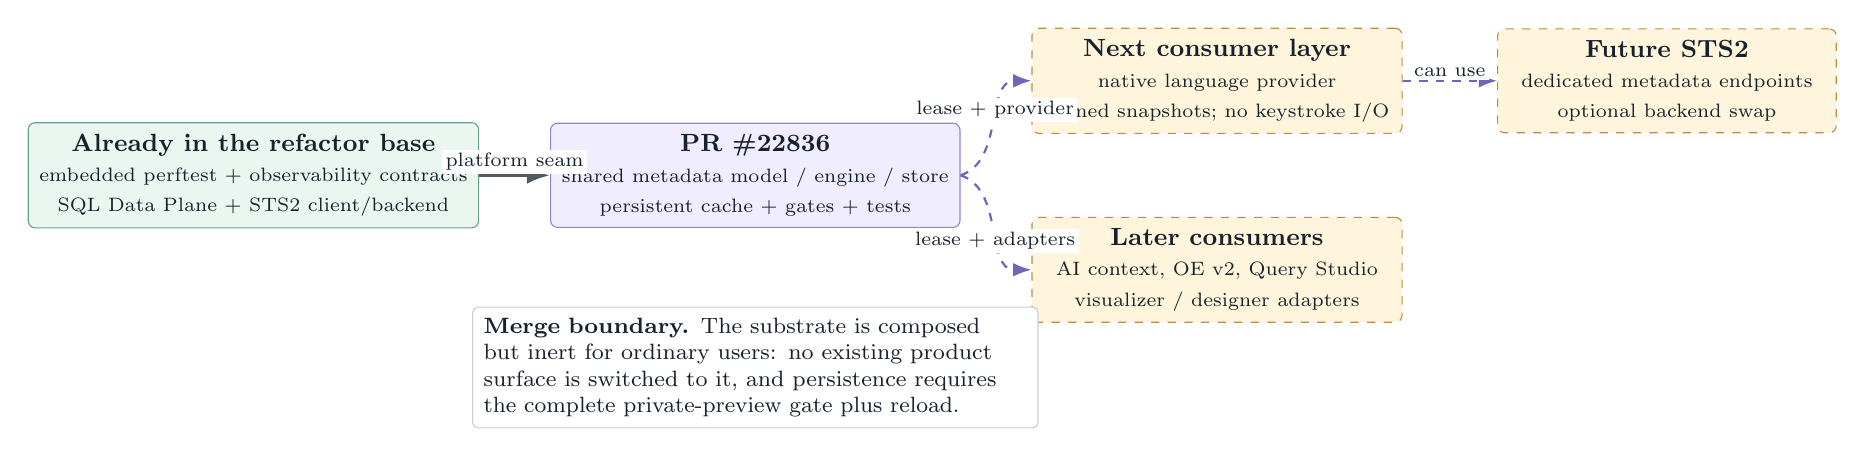
\begin{tikzpicture}[node distance=7mm and 9mm]
  \node[gate,minimum width=44mm] (found) {\textbf{Already in the refactor base}\\\scriptsize embedded perftest + observability contracts\\\scriptsize SQL Data Plane + STS2 client/backend};
  \node[store,minimum width=52mm,right=of found] (pr) {\textbf{PR \#22836}\\\scriptsize shared metadata model / engine / store\\\scriptsize persistent cache + gates + tests};
  \node[planned,minimum width=47mm,right=of pr,yshift=12mm] (ls) {\textbf{Next consumer layer}\\\scriptsize native language provider\\\scriptsize pinned snapshots; no keystroke I/O};
  \node[planned,minimum width=47mm,right=of pr,yshift=-12mm] (ui) {\textbf{Later consumers}\\\scriptsize AI context, OE v2, Query Studio\\\scriptsize visualizer / designer adapters};
  \node[planned,minimum width=43mm,right=12mm of ls] (ep) {\textbf{Future STS2}\\\scriptsize dedicated metadata endpoints\\\scriptsize optional backend swap};

  \draw[arrow] (found) -- node[labelbox,above]{platform seam} (pr);
  \draw[async] (pr.east) to[out=18,in=180] node[labelbox,above]{lease + provider} (ls.west);
  \draw[async] (pr.east) to[out=-18,in=180] node[labelbox,below]{lease + adapters} (ui.west);
  \draw[async] (ls) -- node[labelbox,above]{can use} (ep);

  \node[note,text width=69mm,below=10mm of pr] (boundary) {\textbf{Merge boundary.} The substrate is composed but inert for ordinary users: no existing product surface is switched to it, and persistence requires the complete private-preview gate plus reload.};
\end{tikzpicture}}
\caption{The PR is an enabling layer in the refactor train, not the consumer cutover. Dashed arrows are downstream contracts rather than current product routing.}
\label{fig:train}
\end{figure}

\section{Runtime architecture and composition}

\subsection{One extension-host composition root}

\code{MainController.initializeMetadataStore()} configures host facts and storage before the first store request. \code{MetadataStoreService} lazily creates one \code{MetadataStore} per extension host. The metadata engine itself imports neither VS Code nor the filesystem; focus, poll cadence, data-plane enablement, global-storage path, and settings are injected.

The hierarchy of gates is strict:

\begin{align*}
  \text{cache composed}\iff{}&\ \code{enableExperimentalFeatures} \\
  &\land\ \code{sqlDataPlane.enabled} \\
  &\land\ \code{metadataCache.enabled}.
\end{align*}

All three settings default off where applicable, and changing the dependency path requires a window reload. SQL Data Plane launch arguments also use the private-preview predicate, so merely setting the lower-level flag without the experimental umbrella does not activate STS2.

\begin{figure}[H]
\centering
\resizebox{0.98\textwidth}{!}{%
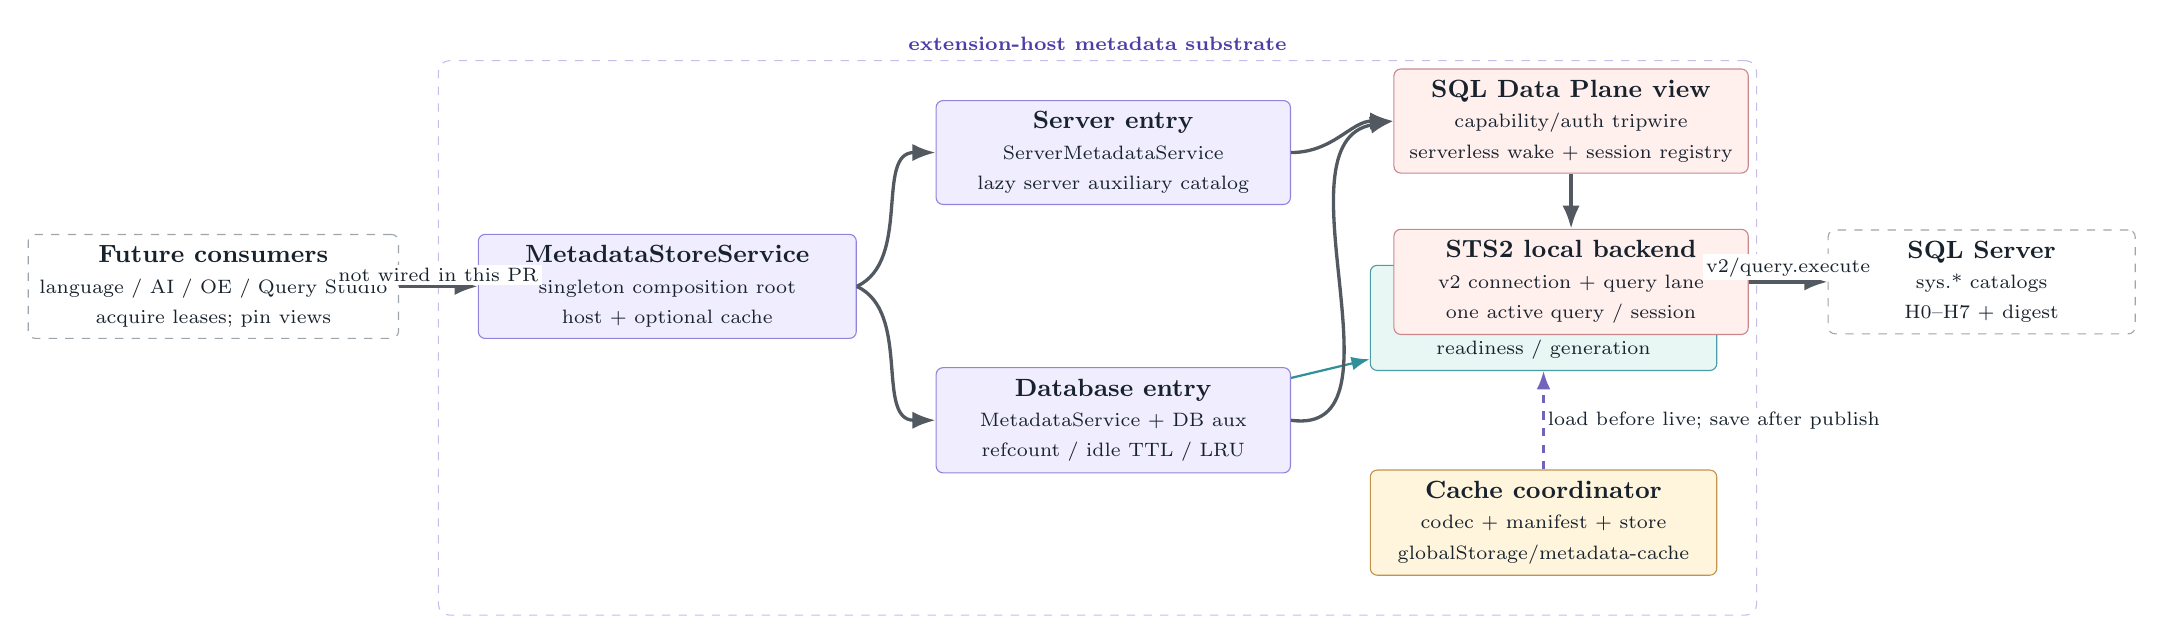
\begin{tikzpicture}[node distance=7mm and 10mm]
  \node[ext,minimum width=43mm] (futureConsumers) {\textbf{Future consumers}\\\scriptsize language / AI / OE / Query Studio\\\scriptsize acquire leases; pin views};
  \node[store,minimum width=48mm,right=of futureConsumers] (root) {\textbf{MetadataStoreService}\\\scriptsize singleton composition root\\\scriptsize host + optional cache};

  \node[store,minimum width=45mm,right=of root,yshift=17mm] (server) {\textbf{Server entry}\\\scriptsize ServerMetadataService\\\scriptsize lazy server auxiliary catalog};
  \node[store,minimum width=45mm,right=of root,yshift=-17mm] (db) {\textbf{Database entry}\\\scriptsize MetadataService + DB aux\\\scriptsize refcount / idle TTL / LRU};

  \node[model,minimum width=44mm,right=of db,yshift=13mm] (snap) {\textbf{CatalogSnapshot}\\\scriptsize immutable SoA + indexes\\\scriptsize readiness / generation};
  \node[cache,minimum width=44mm,right=of db,yshift=-13mm] (disk) {\textbf{Cache coordinator}\\\scriptsize codec + manifest + store\\\scriptsize globalStorage/metadata-cache};

  \node[sess,minimum width=45mm,right=13mm of server,yshift=4mm] (dp) {\textbf{SQL Data Plane view}\\\scriptsize capability/auth tripwire\\\scriptsize serverless wake + session registry};
  \node[sess,minimum width=45mm,below=7mm of dp] (sts) {\textbf{STS2 local backend}\\\scriptsize v2 connection + query lane\\\scriptsize one active query / session};
  \node[ext,minimum width=39mm,right=of sts] (sql) {\textbf{SQL Server}\\\scriptsize sys.* catalogs\\\scriptsize H0--H7 + digest};

  \draw[arrow] (futureConsumers) -- node[labelbox,above]{not wired in this PR} (root);
  \draw[arrow] (root.east) to[out=25,in=180] (server.west);
  \draw[arrow] (root.east) to[out=-25,in=180] (db.west);
  \draw[dataarr] (db) -- (snap);
  \draw[async] (disk) -- node[labelbox,right]{load before live; save after publish} (snap);
  \draw[arrow] (server.east) to[out=0,in=180] (dp.west);
  \draw[arrow] (db.east) to[out=-8,in=190] (dp.west);
  \draw[arrow] (dp) -- (sts);
  \draw[arrow] (sts) -- node[labelbox,above]{v2/query.execute} (sql);

  \begin{scope}[on background layer]
    \node[draw=violet!40,dashed,rounded corners,fit=(root)(server)(db)(snap)(disk),inner sep=5mm,label={[violetdark,font=\scriptsize\bfseries]above:extension-host metadata substrate}] {};
  \end{scope}
\end{tikzpicture}}
\caption{As-built runtime layering. The current transport is generic STS2 query execution; the cache is optional; consumer arrows remain a future integration surface.}
\label{fig:architecture}
\end{figure}

\subsection{Acquisition and the network-authorization boundary}

The acquisition path has two logically separate responsibilities: recover the best local snapshot and, only when policy permits, create live infrastructure. The target ordering is cache-first and network-gated. This matters even when the backend does not open a physical SQL connection immediately: backend startup, polling, strict freshness, and auxiliary calls are all forms of live work that an explicit offline mode must prohibit.

\begin{figure}[H]
\centering
\resizebox{0.98\textwidth}{!}{%
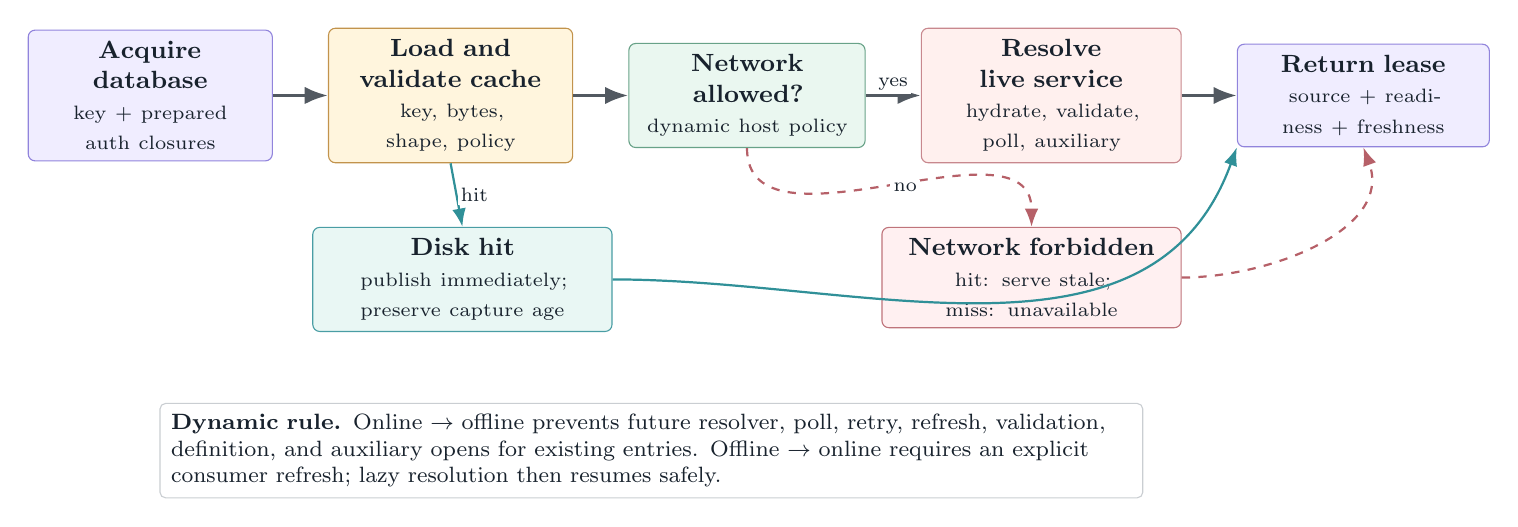
\begin{tikzpicture}[node distance=8mm and 7mm]
  \node[store,text width=28mm,minimum width=31mm] (acq) {\textbf{Acquire database}\\\scriptsize key + prepared auth closures};
  \node[cache,text width=28mm,minimum width=31mm,right=of acq] (load) {\textbf{Load and validate cache}\\\scriptsize key, bytes, shape, policy};
  \node[gate,text width=27mm,minimum width=30mm,right=of load] (net) {\textbf{Network allowed?}\\\scriptsize dynamic host policy};
  \node[sess,text width=30mm,minimum width=33mm,right=of net] (live) {\textbf{Resolve live service}\\\scriptsize hydrate, validate, poll, auxiliary};
  \node[store,text width=29mm,minimum width=32mm,right=of live] (lease) {\textbf{Return lease}\\\scriptsize source + readiness + freshness};

  \node[model,text width=35mm,minimum width=38mm,below left=10mm and 2mm of net] (hit) {\textbf{Disk hit}\\\scriptsize publish immediately; preserve capture age};
  \node[risk,text width=35mm,minimum width=38mm,below right=10mm and 2mm of net] (offline) {\textbf{Network forbidden}\\\scriptsize hit: serve stale; miss: unavailable};

  \draw[arrow] (acq)--(load);
  \draw[arrow] (load)--(net);
  \draw[arrow] (net)--node[labelbox,above]{yes} (live);
  \draw[arrow] (live)--(lease);
  \draw[dataarr] (load.south) -- node[labelbox,right]{hit} (hit.north);
  \draw[dataarr] (hit.east) to[out=0,in=-110] (lease.south west);
  \draw[failarr] (net.south) to[out=-90,in=90] node[labelbox,right]{no} (offline.north);
  \draw[failarr] (offline.east) to[out=0,in=-70] (lease.south);

  \node[note,text width=122mm,below=9mm of hit,xshift=24mm] {\textbf{Dynamic rule.} Online $\rightarrow$ offline prevents future resolver, poll, retry, refresh, validation, definition, and auxiliary opens for existing entries. Offline $\rightarrow$ online requires an explicit consumer refresh; lazy resolution then resumes safely.};
\end{tikzpicture}}
\caption{Implemented acquisition ordering. Offline is a network authorization boundary, not merely ``do not schedule the first background refresh.''}
\label{fig:networkgate}
\end{figure}

\begin{reviewbox}
The repaired store uses a shared lazy provider resolution and passes a live authorization closure into database engines, server engines, and both auxiliary sources. Cache hit, cache miss, explicit refresh, strict freshness, definitions, polling/retry, and online$\rightarrow$offline paths are exercised with resolver/session/query counters. Disposal is rechecked after an asynchronous provider resolution so a late result cannot open a session after ownership ended.
\end{reviewbox}

\subsection{Activation, maintenance, and shutdown}

Composition is deliberately cheap. Cache maintenance is scheduled five seconds after activation and therefore does not contaminate \code{mssql.activate} timing. Debounced cache writes are flushed during extension deactivation before store disposal. Status commands are passive views of already-composed state; the SQL Data Plane status command is designed not to construct a backend or resolve credentials.

The cache-specific commands are:

\begin{itemize}
  \item \code{mssql.metadataCache.showStatus};
  \item \code{mssql.metadataCache.clearAll};
  \item \code{mssql.metadataCache.clearForConnection}; and
  \item explicit enable/disable commands for offline mode.
\end{itemize}

\section{Identity, authentication, and lease lifecycle}

\subsection{Two non-reversible fingerprints}

The store never uses a password, token, or connection string as identity. It JSON-encodes connection-affecting tuples and hashes them with SHA-256, returning a 22-character base64url prefix:

\begin{itemize}
  \item \code{pfp_*}: profile/session identity, including the default database;
  \item \code{sfp_*}: server identity, excluding the database.
\end{itemize}

JSON tuple encoding matters: delimiter-joined fields allow distinct legal values such as \code{["a|b","c"]} and \code{["a","b|c"]} to collide. The current PR fixes and tests this class for both fingerprints and derived profile IDs.

The database store key is \code{serverFingerprint + requested database spelling}. Retaining the spelling is reasonable before the catalog comparison rule is known, but it creates an obligation: the live session must prove that the database it opened is the database represented by the key before any snapshot or cache write is published.

\subsection{Secrets stay deferred}

\code{prepareConnection()} produces a sanitized profile reference and closures for authentication:

\begin{itemize}
  \item SQL passwords are read from the credential store only when a physical session open requires them;
  \item Entra tokens are acquired only at physical open;
  \item integrated authentication carries no secret provider.
\end{itemize}

The SQL Data Plane registry evaluates declared requirements before invoking credential closures. The repaired public service view is the single Azure serverless wake owner; top-level \code{openSession()} delegates through that view once. Static requirement failures remain non-retryable capability errors, while a live provider \code{canOpen()} refusal becomes retryable \code{unavailable}. This keeps capability checking, credential deferral, provider availability, and wake ownership separate.

\subsection{Single-flight entries and ref-counted leases}

First acquisition is single-flight per key for both server and database entries. Concurrent same-key callers join one creation rather than producing orphan engines or sessions. Each lease increments a refcount; disposal decrements it idempotently. A zero-ref database remains warm for a bounded idle period, and the least recently released idle entry is disposed first when the cap is exceeded.

A database entry owns:

\begin{itemize}
  \item one session source for serialized hydration, digest validation, and lazy module definitions;
  \item one separate source for database auxiliary sections;
  \item one metadata engine, one lease handle, listeners, and cache-source state.
\end{itemize}

The resource split keeps ordinary metadata work away from user query sessions. A catalog-wide FIFO lane now serializes different auxiliary section keys around session open and query completion, while same-section callers still coalesce. The deterministic fake-backend regression starts two distinct sections together and proves both complete through one STS2-compatible one-active-query session.

\subsection{Fail-closed database identity and recovery}

The target identity protocol has two stages. The returned session metadata is a preliminary signal; H0's \code{DB_NAME()} plus \code{CATALOG_DEFAULT} comparison behavior is the authoritative proof. No H1--H7 rows should publish until that proof succeeds. A timeout or later rename drift must fence the current operation epoch, recycle the physical source, and reopen by the requested database name before clearing the drift latch.

\begin{figure}[H]
\centering
\resizebox{0.96\textwidth}{!}{%
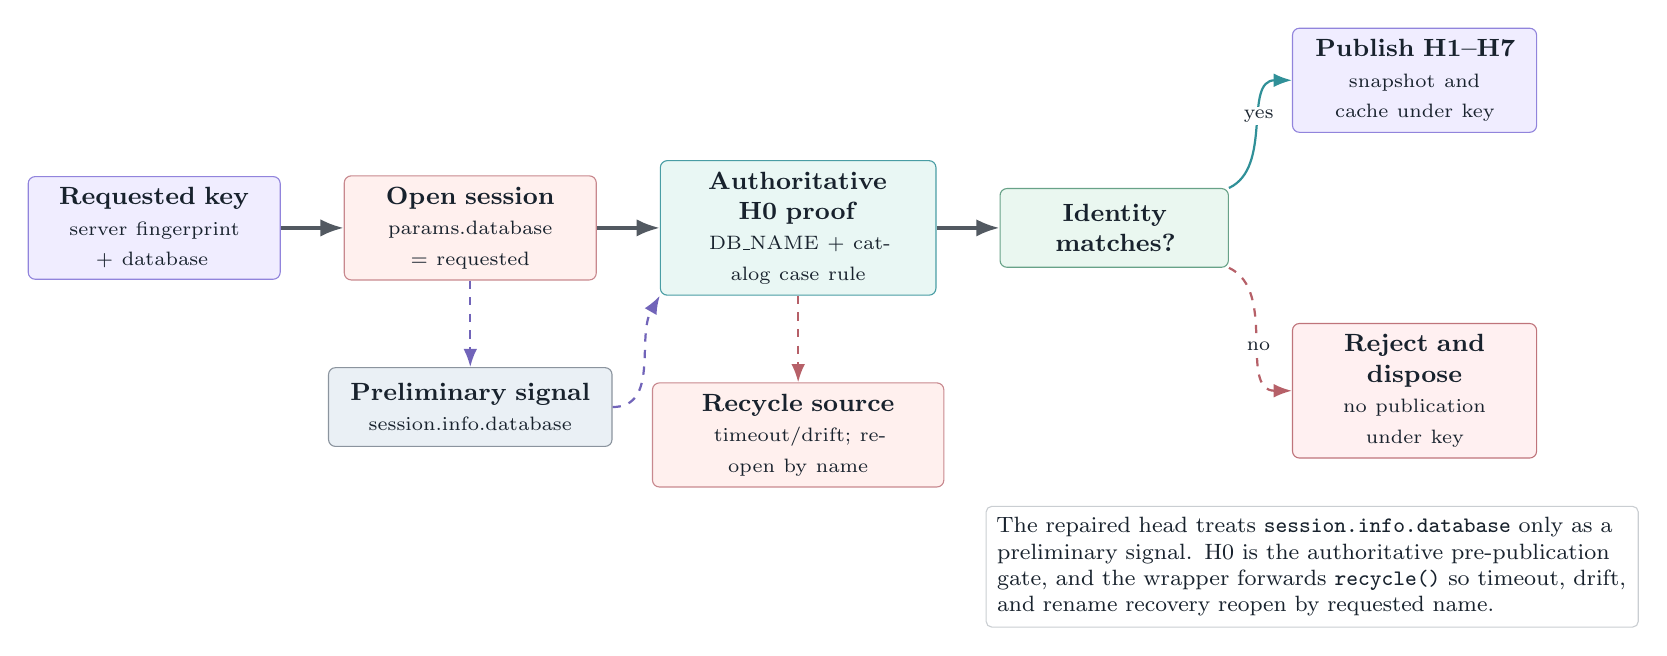
\begin{tikzpicture}[node distance=9mm and 8mm]
  \node[store,text width=29mm,minimum width=32mm] (key) {\textbf{Requested key}\\\scriptsize server fingerprint + database};
  \node[sess,text width=29mm,minimum width=32mm,right=of key] (open) {\textbf{Open session}\\\scriptsize params.database = requested};
  \node[model,text width=32mm,minimum width=35mm,right=of open] (h0) {\textbf{Authoritative H0 proof}\\\scriptsize DB\_NAME + catalog case rule};
  \node[gate,text width=26mm,minimum width=29mm,right=of h0] (gate) {\textbf{Identity matches?}};
  \node[store,text width=28mm,minimum width=31mm,above right=7mm and 8mm of gate] (publish) {\textbf{Publish H1--H7}\\\scriptsize snapshot and cache under key};
  \node[risk,text width=28mm,minimum width=31mm,below right=7mm and 8mm of gate] (reject) {\textbf{Reject and dispose}\\\scriptsize no publication under key};
  \node[comp,text width=33mm,minimum width=36mm,below=11mm of open] (pre) {\textbf{Preliminary signal}\\\scriptsize session.info.database};
  \node[sess,text width=34mm,minimum width=37mm,below=11mm of h0] (recycle) {\textbf{Recycle source}\\\scriptsize timeout/drift; reopen by name};

  \draw[arrow] (key)--(open);
  \draw[arrow] (open)--(h0);
  \draw[arrow] (h0)--(gate);
  \draw[dataarr] (gate.north east) to[out=25,in=180] node[labelbox,above]{yes} (publish.west);
  \draw[failarr] (gate.south east) to[out=-25,in=180] node[labelbox,below]{no} (reject.west);
  \draw[async] (open.south)--(pre.north);
  \draw[async] (pre.east) to[out=0,in=-120] (h0.south west);
  \draw[failarr] (h0.south)--(recycle.north);

  \node[note,text width=80mm,below=6mm of reject,xshift=-13mm] {The repaired head treats \code{session.info.database} only as a preliminary signal. H0 is the authoritative pre-publication gate, and the wrapper forwards \code{recycle()} so timeout, drift, and rename recovery reopen by requested name.};
\end{tikzpicture}}
\caption{Database identity must be a publication gate. Detection without rejection is observability, not key correctness.}
\label{fig:identitygate}
\end{figure}

\begin{reviewbox}
This gate is implemented, not aspirational: the wrapper forwards \code{recycle: () => inner.recycle()}, and authoritative H0 identity must match the requested key under the catalog comparison rule before H1 or cache publication. Tests cover a backend that ignores \code{params.database}, case-insensitive spelling variation, a true mismatch, and watchdog recovery proving that the next operation uses a fresh session.
\end{reviewbox}

\section{Catalog model: compact truth with explicit unknowns}

\subsection{Structure of arrays and immutable publication}

\code{CatalogBuilder} interns strings and appends parallel arrays for schemas, objects, columns, keys, foreign keys, parameters, descriptions, and exact details. An object-id index makes row ingestion constant-time per row. \code{CatalogSnapshot} builds read-only indexes over those arrays and exposes query methods, not mutation.

This design has three consequences:

\begin{enumerate}
  \item repeated schema/object/type names occupy one string-table entry;
  \item canonical array order is directly serializable and hashable; and
  \item a published generation is internally consistent because readers never observe a partially mutated model.
\end{enumerate}

The exact detail surface includes stable \code{column_id}, type schema/base type, system and user type IDs, UDT/assembly flags, raw max length in bytes, precision/scale, collation, default definition, exact-text identity seed/increment, computed definition/persistence, FK constraint IDs, referential actions, column-pair ordinals, and endpoint column IDs. Defaults and computed definitions are live structural detail but are stripped before persistence.

\subsection{Readiness is per section}

Each section is one of \code{absent}, \code{loading}, \code{ready}, \code{failed}, \code{stale}, or \code{lite}. The snapshot also carries \code{full}, \code{partial}, or \code{lite} mode. The distinction is semantic:

\begin{itemize}
  \item \code{absent}: not hydrated or intentionally excluded;
  \item \code{failed}: attempted but unavailable;
  \item \code{lite}: useful identity-level data but not the complete contract;
  \item \code{stale} in readiness: a transient rehydration state over an existing snapshot, \emph{not} age-based staleness.
\end{itemize}

Age and validation are represented by the freshness result described in \cref{sec:freshness}. This prevents one overloaded boolean from lying about both completeness and recency.

\subsection{Progressive hydration ladder}

\begin{table}[H]
\centering
\small
\caption{The live database hydration ladder at the pinned PR head.}
\label{tab:hydration}
\begin{tabularx}{\textwidth}{@{}p{0.075\textwidth}p{0.19\textwidth}X@{}}
\toprule
\textbf{Step} & \textbf{Section/fact} & \textbf{Important behavior}\\
\midrule
H0 & Environment & Engine edition, default schema, database collation, \code{CATALOG_DEFAULT} case rule, canonical \code{DB_NAME()}. Current fallback silently uses case-insensitive lookup when the probe fails; the safer contract is unknown/exact-only or an unavailable name-resolution section.\\
H1 & Schemas & All visible \code{sys.schemas}; no high-ID role-schema filter.\\
H2 & Objects & User tables, views, procedures, scalar/table functions, synonyms, CLR routines/aggregates; system-shipped rows excluded.\\
H3 & Columns/details & Visible columns only; hidden temporal/graph implementation columns excluded; exact type/default/identity/computed facts retained live.\\
H4 & PK/UQ & Primary-key and unique-constraint columns in key ordinal order.\\
H5/H5B & Foreign keys & Enabled FKs, including untrusted-but-enforced constraints; referential actions and ordered column pairs; invisible endpoints are not published as dangling edges.\\
H6 & Parameters & Routine parameters and return value ordinal 0; schema-qualified UDT display retains exact spelling.\\
H7 & Descriptions & Object/column \code{MS_Description} values, failure-visible and live-only under current persistence policy.\\
\bottomrule
\end{tabularx}
\end{table}

Synonyms are honestly \code{lite}: identity is present, target traversal is not. The \code{types} section is \code{absent}: table-type shapes and sequences remain a downstream model enrichment. Module text is not part of H0--H7; \code{getModuleDefinition(objectId)} performs one safe-integer-checked, lazy \code{sys.sql_modules} query and caches it only for the current generation.

\subsection{Server and auxiliary catalogs}

The server service hydrates environment and database-list facts independently from database catalogs. Additional server and database folders use \code{AuxiliaryCatalog}: a keyed table of lazy sections with single-flight hydration and per-section refresh. This is the extension point for security, broker, storage, programmability leaves, logins, roles, credentials, endpoints, system objects, and designer facets without bloating connect-time hydration.

Auxiliary queries use sources separate from the main hydration lane, which is the correct resource boundary. The repaired auxiliary engine retains same-section coalescing and adds a catalog-wide FIFO promise lane around \code{sessions.open()} plus \code{runMetadataQuery()}, so different section keys cannot overlap on one cached STS2 session. Names returned by auxiliary sections remain outside diagnostic events.

\subsection{Deterministic schema context}

\code{buildSchemaContext()} produces bounded text from a pinned snapshot for AI or language consumers. Ordering uses an ordinal, locale-independent comparator: Unicode-default fold followed by a raw code-unit tiebreak. This avoids Electron/ICU-version drift and preserves case-distinct names. The selection algorithm precomputes FK degree, renders each candidate at most once per fidelity tier, and takes a prefix that fits the character budget; the former quadratic shrink-and-rerender path is now linear in catalog size per tier.

\begin{figure}[H]
\centering
\resizebox{0.96\textwidth}{!}{%
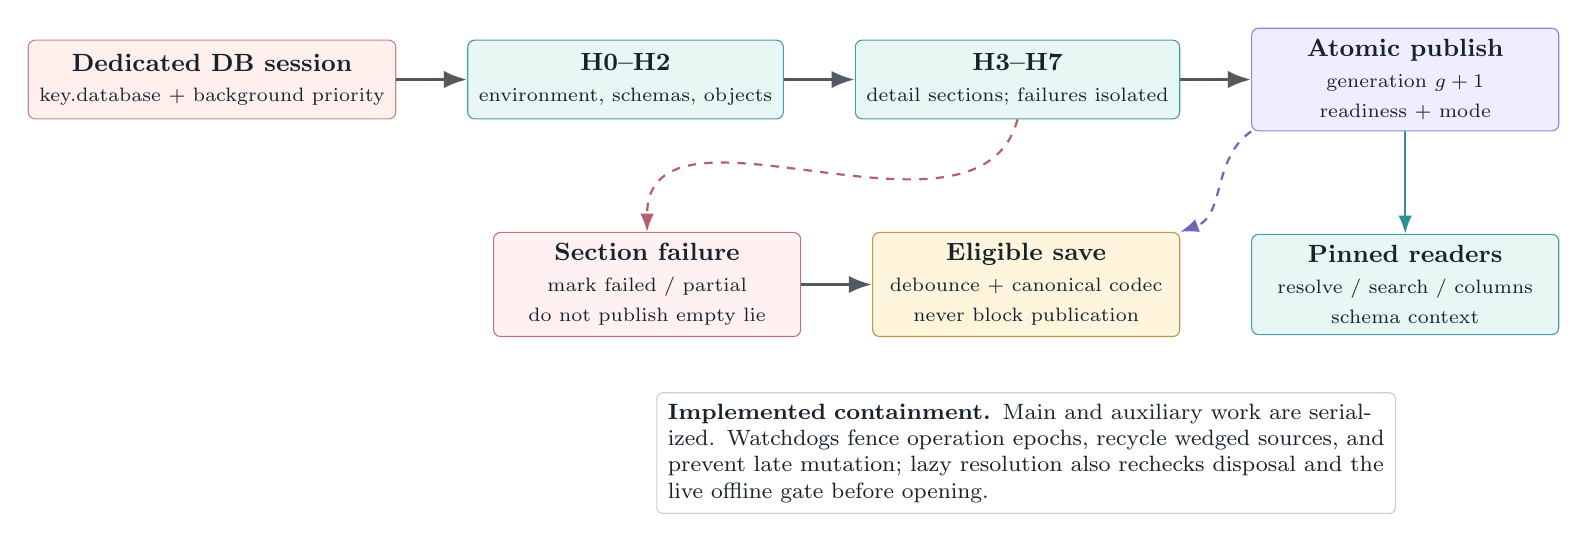
\begin{tikzpicture}[node distance=7mm and 9mm]
  \node[sess,minimum width=38mm] (open) {\textbf{Dedicated DB session}\\\scriptsize key.database + background priority};
  \node[model,minimum width=39mm,right=of open] (h0) {\textbf{H0--H2}\\\scriptsize environment, schemas, objects};
  \node[model,minimum width=39mm,right=of h0] (h3) {\textbf{H3--H7}\\\scriptsize detail sections; failures isolated};
  \node[store,minimum width=39mm,right=of h3] (publish) {\textbf{Atomic publish}\\\scriptsize generation $g+1$\\\scriptsize readiness + mode};

  \node[model,minimum width=39mm,below=13mm of publish] (readers) {\textbf{Pinned readers}\\\scriptsize resolve / search / columns\\\scriptsize schema context};
  \node[cache,minimum width=39mm,left=of readers] (save) {\textbf{Eligible save}\\\scriptsize debounce + canonical codec\\\scriptsize never block publication};
  \node[risk,minimum width=39mm,left=of save] (failure) {\textbf{Section failure}\\\scriptsize mark failed / partial\\\scriptsize do not publish empty lie};

  \draw[arrow] (open)--(h0);
  \draw[arrow] (h0)--(h3);
  \draw[arrow] (h3)--(publish);
  \draw[dataarr] (publish)--(readers);
  \draw[async] (publish.south west) to[out=-145,in=20] (save.north east);
  \draw[failarr] (h3.south) to[out=-105,in=90] (failure.north);
  \draw[arrow] (failure.east)--(save.west);

  \node[note,text width=91mm,below=7mm of save] {\textbf{Implemented containment.} Main and auxiliary work are serialized. Watchdogs fence operation epochs, recycle wedged sources, and prevent late mutation; lazy resolution also rechecks disposal and the live offline gate before opening.};
\end{tikzpicture}}
\caption{Rows are accumulated privately and published as one immutable generation. Per-section failure truth survives publication and persistence eligibility.}
\label{fig:hydrate}
\end{figure}

\section{Freshness, drift, and polling}\label{sec:freshness}

\subsection{Consumers state a policy, not an implementation}

The freshness API decouples consumer intent from cache and network mechanics. A request declares a mode, reason, optional required sections/objects, staleness or validation TTL, partial-data tolerance, disk-load permission, background-refresh preference, and a wait/abort budget.

\begin{table}[H]
\centering
\small
\caption{Freshness modes and their honest outcomes.}
\label{tab:freshness}
\begin{tabularx}{\textwidth}{@{}p{0.19\textwidth}p{0.25\textwidth}X@{}}
\toprule
\textbf{Mode} & \textbf{Normal use} & \textbf{Decision semantics}\\
\midrule
\code{allowStale} & completion, AI context & Return any snapshot immediately; optionally start background refresh. With no snapshot, join hydration only up to the caller's budget.\\
\code{requireValidated} & diagnostics, OE browse & Accept a recent validation TTL; otherwise coalesce a cheap digest. Unchanged means validated; changed chains a full refresh. Timeout returns best snapshot as stale/unavailable, never cancels shared work.\\
\code{requireLive} & scripting or destructive/fidelity-sensitive work & Join/start a forced refresh. Failure, timeout, or identity drift returns \code{unavailable}; a retained snapshot may still ride in the result for an explicit offline choice.\\
\code{offlineSnapshot} & user-selected offline operation & Perform no backend resolution, SQL session open, poll, validation, refresh, or auxiliary query. Return disk/memory snapshot as stale with age, or unavailable if none exists. The live store/engine/server/auxiliary gate enforces the same rule after an online$\rightarrow$offline transition.\\
\bottomrule
\end{tabularx}
\end{table}

Freshness results distinguish \code{live}, \code{validated}, \code{refreshing}, \code{stale}, and \code{unavailable}; they also carry source, generation, capture time, stale age, wait time, validation summary, and whether background work started. Section readiness is checked \emph{after} the freshness decision. A strict caller requiring columns cannot accept a fresh snapshot whose columns section failed.

\begin{figure}[H]
\centering
\resizebox{\textwidth}{!}{%
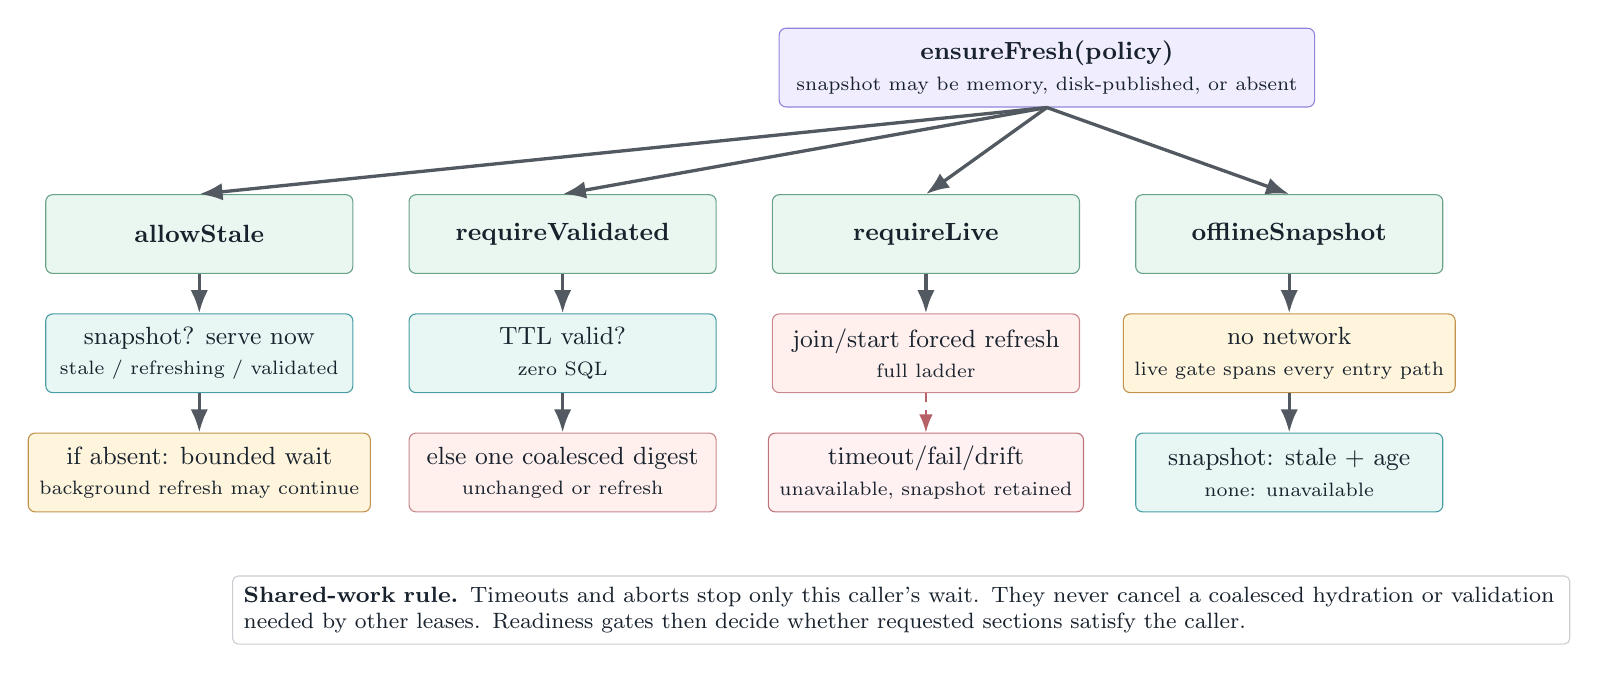
\begin{tikzpicture}[node distance=5mm and 7mm]
  \node[store,minimum width=68mm] (entry) {\textbf{ensureFresh(policy)}\\\scriptsize snapshot may be memory, disk-published, or absent};

  \node[gate,minimum width=39mm,below left=11mm and 54mm of entry] (stale) {\textbf{allowStale}};
  \node[gate,minimum width=39mm,right=of stale] (validated) {\textbf{requireValidated}};
  \node[gate,minimum width=39mm,right=of validated] (live) {\textbf{requireLive}};
  \node[gate,minimum width=39mm,right=of live] (offline) {\textbf{offlineSnapshot}};
  \foreach \n in {stale,validated,live,offline} {\draw[arrow] (entry.south) -- (\n.north);}

  \node[model,minimum width=39mm,below=of stale] (s1) {snapshot? serve now\\\scriptsize stale / refreshing / validated};
  \node[cache,minimum width=39mm,below=of s1] (s2) {if absent: bounded wait\\\scriptsize background refresh may continue};
  \draw[arrow] (stale)--(s1); \draw[arrow] (s1)--(s2);

  \node[model,minimum width=39mm,below=of validated] (v1) {TTL valid?\\\scriptsize zero SQL};
  \node[sess,minimum width=39mm,below=of v1] (v2) {else one coalesced digest\\\scriptsize unchanged or refresh};
  \draw[arrow] (validated)--(v1); \draw[arrow] (v1)--(v2);

  \node[sess,minimum width=39mm,below=of live] (l1) {join/start forced refresh\\\scriptsize full ladder};
  \node[risk,minimum width=39mm,below=of l1] (l2) {timeout/fail/drift\\\scriptsize unavailable, snapshot retained};
  \draw[arrow] (live)--(l1); \draw[failarr] (l1)--(l2);

  \node[cache,minimum width=39mm,below=of offline] (o1) {no network\\\scriptsize live gate spans every entry path};
  \node[model,minimum width=39mm,below=of o1] (o2) {snapshot: stale + age\\\scriptsize none: unavailable};
  \draw[arrow] (offline)--(o1); \draw[arrow] (o1)--(o2);

  \node[note,text width=167mm,below=8mm of v2,xshift=43mm] {\textbf{Shared-work rule.} Timeouts and aborts stop only this caller's wait. They never cancel a coalesced hydration or validation needed by other leases. Readiness gates then decide whether requested sections satisfy the caller.};
\end{tikzpicture}}
\caption{The freshness decision has four modes but one invariant: return the best snapshot with an explicit truth label; never silently elevate stale or partial data.}
\label{fig:freshness}
\end{figure}

\subsection{Three drift paths}

\textbf{Local DDL sniff.} After a successful executed batch, a leading-keyword lexer recognizes \code{CREATE}, \code{ALTER}, \code{DROP}, and \code{SP_RENAME}; \code{EXEC}/\code{EXECUTE} trigger a conservative digest check. A burst while hydration is active collapses to at most one follow-up refresh.

\textbf{Cheap digest.} The T1 query hashes visible object count plus object ID, schema ID, byte-exact name, and modify date. Including schema and binary name fixes the classic \code{sp_rename}/\code{ALTER SCHEMA TRANSFER} blind spot. It remains evidence of likely equality, not proof: column/key/FK/parameter-only drift awaits future section/object digests or an explicit refresh.

\textbf{Explicit policy.} A strict consumer can force validation or a full live refresh. This is the correctness backstop when polling is disabled, suspended, or intentionally sparse.

\subsection{Poll governance}

The default base interval is 60 seconds with multipliers \(1,2,5\) and independent \(\pm 10\%\) jitter. Consecutive unchanged verdicts back off; refresh or detected activity resets to base. Validation fan-out is capped at two per server fingerprint, so one sleeping server cannot starve another and a resume event cannot open dozens of digest queries against one server.

After two minutes unfocused, polling suspends without SQL. Refocus schedules immediate, limiter-bounded validation and re-jitters timers. Azure SQL Database and Synapse serverless engine editions (5 and 11) poll at the cap so a background digest is less likely to defeat auto-pause; consumer activity still invokes TTL validation. Setting \code{mssql.metadata.pollSeconds=0} disables polling.

\section{Persistent cache design}

\subsection{Purpose, defaults, and trust boundary}

The cache reduces first-use latency and supports explicit offline browsing; it is not the source of authority. It is off by default, stored under the extension's local or remote \code{globalStorage/metadata-cache/v1}, limited by default to 14 days, 256 MiB total, and 32 MiB compressed per entry, with a five-second save debounce.

A cache entry is attacker-shaped or corruption-shaped local input. The read path must therefore prove four independent properties before publication:

\begin{enumerate}
  \item \textbf{key ownership}: the manifest belongs to the requested server/database key;
  \item \textbf{physical integrity}: referenced compressed bytes exist, fit bounds, and match SHA-256;
  \item \textbf{logical integrity}: decoded canonical content matches the manifest's content hash and structural invariants;
  \item \textbf{policy compatibility}: privacy/readiness is intersected with current settings rather than elevated.
\end{enumerate}

The repaired implementation verifies all four properties. Requested server fingerprint, derived database hash, and optional exact database spelling must match before adoption; decoded payloads are canonicalized and re-hashed after shape validation. Mismatch is a classified safe miss with best-effort quarantine.

\subsection{Canonical payload and manifest}

The \code{cm2} payload is canonical-order JSON over environment, interned strings, and structure-of-arrays fields, gzip-compressed. A model-version change is a clean miss rather than an in-place migration. Two hashes serve different jobs:

\begin{itemize}
  \item manifest \code{payload.sha256}: full SHA-256 of the compressed payload file;
  \item \code{contentHash}: \code{csh_} plus a truncated base64url SHA-256 of canonical uncompressed JSON, intended to identify logical equality across processes/compressions.
\end{itemize}

The manifest records producer versions, writer ID, server fingerprint, database hash and optional exact database name, capture/generation/source, validation summary, environment, readiness, mode, counts/sizes, privacy policy, and the content-addressed payload filename.

\begin{reviewbox}[title={Manifest key binding}]
\code{readEntry(key)} now compares \code{manifest.key.serverFingerprint}, \code{databaseHash}, and optional \code{databaseExact} with the requested key. The regression copies a fully valid A entry into B's already-derived directory and proves B returns \code{keyMismatch} and invalidates the manifest rather than adopting A's catalog.
\end{reviewbox}

\subsection{Privacy intersection}

Current declared settings force description and module-definition persistence off. The codec strips default/computed SQL definitions before writing, and row counts are absent. The disk payload therefore contains structural catalog facts: schema/object/column/type/key/FK/parameter identities and exact non-definition facets.

Load applies policy intersection in both directions. A section disallowed by current policy, absent from payload, or never supported in v1 becomes \code{absent}; it never becomes ready-but-empty. A policy-ID mismatch is a normal intersected hit, not corruption.

\begin{warningbox}
``Hashed paths'' are not encryption. The manifest may contain the exact database name, and the payload contains structural names and types. This is sanctioned local metadata, potentially sensitive, under VS Code global storage. The contract is exclusion, integrity, boundedness, and safe diagnostics---not confidentiality from a user or process that can read the directory.
\end{warningbox}

\subsection{Read protocol}

A reader begins with the manifest because it is the trust root. It validates format/codec/model/shape, resolves the content-addressed payload, checks actual compressed size, verifies SHA-256, enforces a hard decompressed bound during gunzip, parses JSON, validates parallel-array and referential invariants, intersects policy, adopts arrays, and preserves the original capture time/generation.

\begin{figure}[H]
\centering
\resizebox{0.95\textwidth}{!}{%
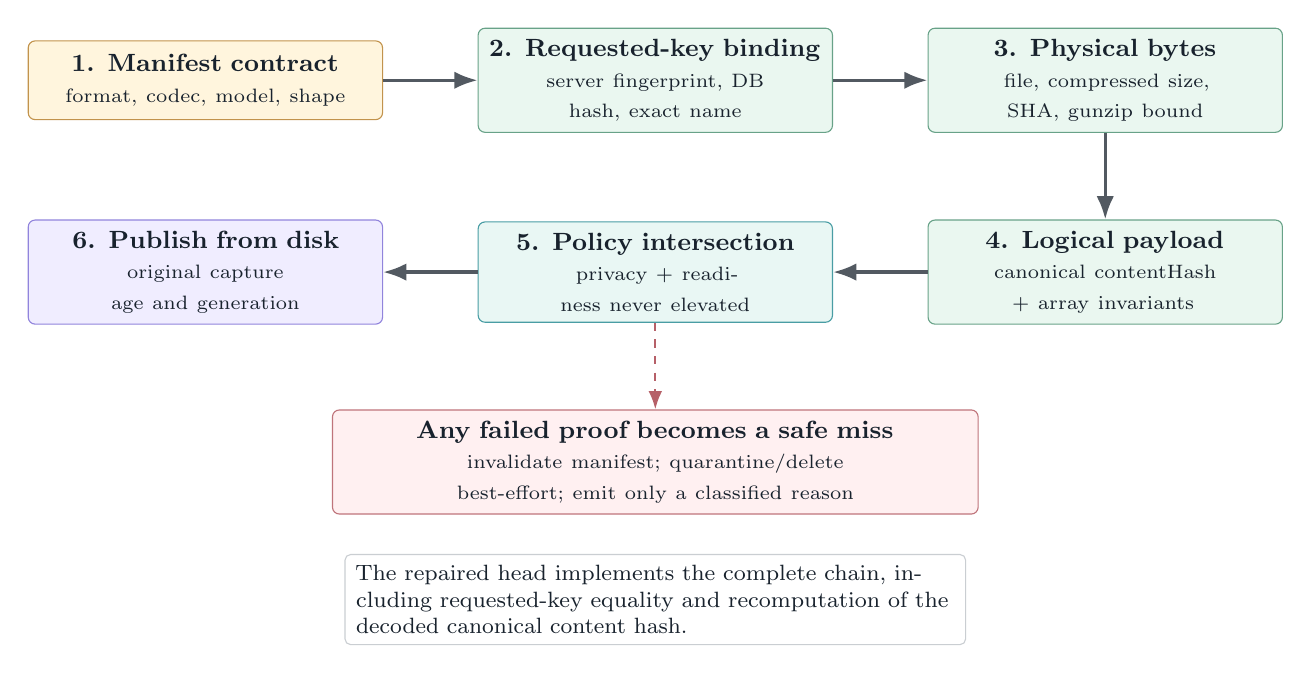
\begin{tikzpicture}[node distance=8mm and 12mm]
  \node[cache,text width=42mm,minimum width=45mm] (manifest) {\textbf{1. Manifest contract}\\\scriptsize format, codec, model, shape};
  \node[gate,text width=42mm,minimum width=45mm,right=of manifest] (key) {\textbf{2. Requested-key binding}\\\scriptsize server fingerprint, DB hash, exact name};
  \node[gate,text width=42mm,minimum width=45mm,right=of key] (bytes) {\textbf{3. Physical bytes}\\\scriptsize file, compressed size, SHA, gunzip bound};

  \node[gate,text width=42mm,minimum width=45mm,below=11mm of bytes] (logical) {\textbf{4. Logical payload}\\\scriptsize canonical contentHash + array invariants};
  \node[model,text width=42mm,minimum width=45mm,left=of logical] (policy) {\textbf{5. Policy intersection}\\\scriptsize privacy + readiness never elevated};
  \node[store,text width=42mm,minimum width=45mm,left=of policy] (publish) {\textbf{6. Publish from disk}\\\scriptsize original capture age and generation};

  \node[risk,text width=78mm,minimum width=82mm,below=11mm of policy] (miss) {\textbf{Any failed proof becomes a safe miss}\\\scriptsize invalidate manifest; quarantine/delete best-effort; emit only a classified reason};

  \draw[arrow] (manifest)--(key); \draw[arrow] (key)--(bytes);
  \draw[arrow] (bytes.south)--(logical.north);
  \draw[arrow] (logical)--(policy); \draw[arrow] (policy)--(publish);
  \draw[failarr] (policy.south)--(miss.north);

  \node[note,text width=76mm,below=5mm of miss] {The repaired head implements the complete chain, including requested-key equality and recomputation of the decoded canonical content hash.};
\end{tikzpicture}}
\caption{Complete cache trust chain. A structurally valid manifest is not trusted merely because it sits in the expected directory.}
\label{fig:cachetrust}
\end{figure}

\subsection{Write protocol and cross-window authority}

Payloads are content-addressed. A writer serializes and compresses, checks the cap, writes a same-directory temporary file with fsync, renames the payload into place, then writes and renames the manifest last. Transient Windows rename failures retry with bounded jitter. Content addressing prevents a manifest from accidentally referring to another writer's bytes with the same fixed filename.

Content addressing does not, by itself, decide which capture is authoritative. The repaired coordinator adds an exclusive-create per-key publication lock around re-read, authority comparison, payload/manifest commit, and postcheck. Authority uses the globally comparable capture instant, never a process-local generation; equal-instant unequal payloads use the ordinal content hash as a deterministic tie-break.

\begin{figure}[H]
\centering
\resizebox{0.94\textwidth}{!}{%
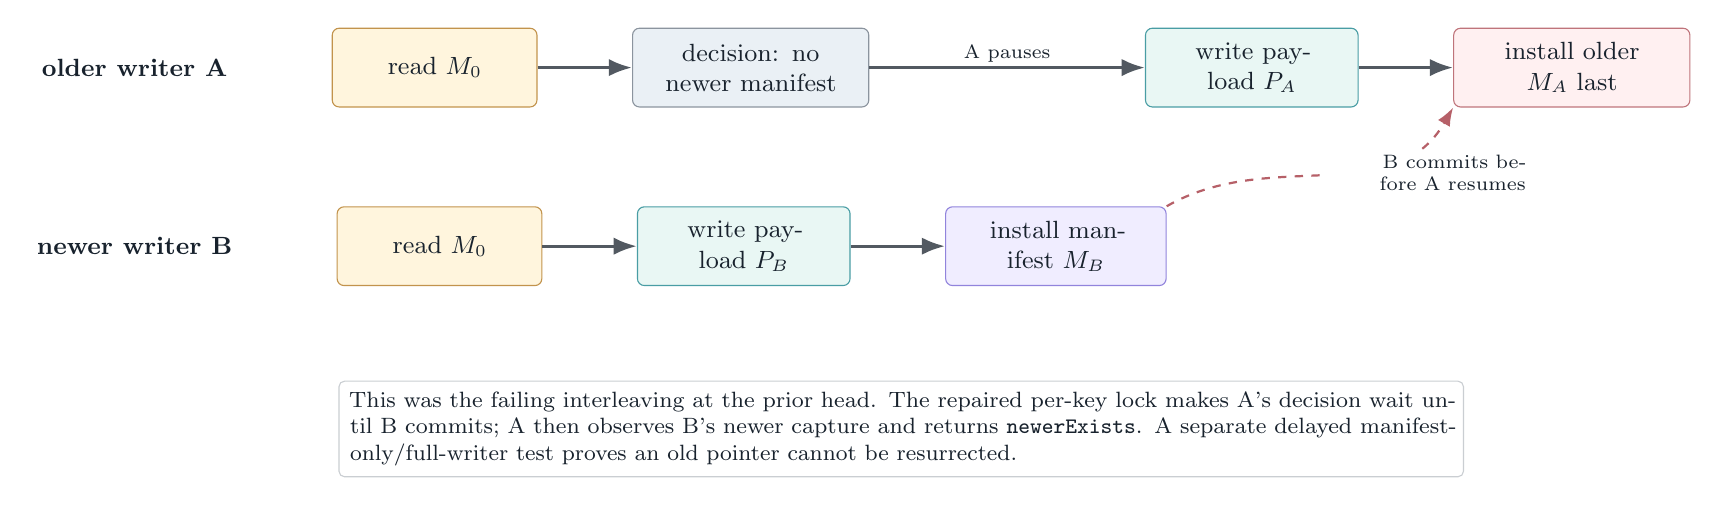
\begin{tikzpicture}[node distance=9mm and 12mm]
  \node[font=\small\bfseries] (alabel) {older writer A};
  \node[cache,text width=23mm,minimum width=26mm,right=of alabel] (a1) {read $M_0$};
  \node[comp,text width=27mm,minimum width=30mm,right=of a1] (a2) {decision: no newer manifest};
  \node[model,text width=24mm,minimum width=27mm,right=35mm of a2] (a3) {write payload $P_A$};
  \node[risk,text width=27mm,minimum width=30mm,right=of a3] (a4) {install older $M_A$ last};

  \node[font=\small\bfseries,below=18mm of alabel] (blabel) {newer writer B};
  \node[cache,text width=23mm,minimum width=26mm,right=of blabel] (b1) {read $M_0$};
  \node[model,text width=24mm,minimum width=27mm,right=of b1] (b2) {write payload $P_B$};
  \node[store,text width=25mm,minimum width=28mm,right=of b2] (b3) {install manifest $M_B$};

  \draw[arrow] (a1)--(a2);
  \draw[arrow] (a2)--node[labelbox,above]{A pauses} (a3);
  \draw[arrow] (a3)--(a4);
  \draw[arrow] (b1)--(b2); \draw[arrow] (b2)--(b3);
  \draw[failarr] (b3.north east) to[out=30,in=-120]
    node[labelbox,right,text width=31mm]{B commits before A resumes}
    (a4.south west);

  \node[note,text width=140mm,below=12mm of b2,xshift=20mm] {This was the failing interleaving at the prior head. The repaired per-key lock makes A's decision wait until B commits; A then observes B's newer capture and returns \code{newerExists}. A separate delayed manifest-only/full-writer test proves an old pointer cannot be resurrected.};
\end{tikzpicture}}
\caption{Formerly unsafe two-window interleaving, now retained as a deterministic regression. Content addressing protects bytes; the per-key critical section protects authority.}
\label{fig:cacheinterleave}
\end{figure}

\begin{table}[H]
\centering
\small
\caption{Required cache publication properties.}
\label{tab:cachepublication}
\begin{tabularx}{\textwidth}{@{}p{0.30\textwidth}p{0.28\textwidth}X@{}}
\toprule
\textbf{Property} & \textbf{Repaired mechanism} & \textbf{Closure evidence}\\
\midrule
Payload/manifest byte coherence & Content-addressed payload + manifest-last + SHA & Strong; retain bounded manifest re-read for reader/writer races.\\
Newer capture cannot be overwritten & Exclusive per-key lock + capture-time authority + deterministic equal-time hash tie-break & Reverse-order older/newer writer regression; newer capture remains authoritative even with lower local generation.\\
Manifest-only update cannot resurrect stale pointer & Equality proof and manifest rewrite occur under the same lock using a fully validated payload & Delayed old manifest-only writer interleaves with a newer full writer; new payload remains readable.\\
Logical equality is trustworthy & Decoded canonical \code{contentHash} is recomputed before adoption or manifest-only equality & Valid compressed bytes and shape with a false logical hash are rejected as corrupt.\\
Reader key isolation & Manifest key fields are compared explicitly to the requested key & Valid A entry copied into B's directory returns \code{keyMismatch}.\\
\bottomrule
\end{tabularx}
\end{table}

\subsection{Eviction, clearing, and index status}

Maintenance coalesces re-entrant calls and throttles filesystem operations. Removal order is corrupt/unsupported and aged entries first, then least-recently-used entries until bytes fit. Manifest-less payloads, old temporary files, quarantine files, and superseded payloads receive an orphan grace. Clears remove manifests first, making remaining bytes inert before deleting payloads.

The JSON index is a convenience cache for listing/access/LRU rather than the trust root. Each window may still lose an access tick while replacing the whole index; source documentation now calls cross-window access/LRU approximate. Manifests remain authoritative for identity and content, and maintenance rebuilds membership and byte totals. Serializing this advisory file with catalog publication would widen a correctness-critical lock for no catalog-safety gain, so this limitation is accepted rather than hidden.

\section{Language-service fit}

\subsection{The contract supplied by this PR}

The future native language engine needs stable environment and catalog views, not direct knowledge of cache files, SQL sessions, or mutable hydration. The metadata substrate supplies the raw ingredients:

\begin{itemize}
  \item environment: current/default database/schema, catalog case behavior, engine edition, collation;
  \item name resolution: exact/default-schema/ambiguous/not-found/section-unavailable;
  \item schemas, objects, columns, keys, FKs, parameters, descriptions, search and system/auxiliary projections;
  \item a generation that invalidates per-request derived caches; and
  \item explicit readiness/freshness so diagnostics can suppress instead of hallucinating.
\end{itemize}

The language-service design in the notes adds a thin provider interface and an \code{IPinnedMetadataView}. That provider should adapt \code{CatalogSnapshot} without exposing implementation classes. Every feature request pins once; all synchronous completion/binding operations read that generation only. Lazy module definitions remain the exceptional asynchronous resolve path.

\subsection{No network I/O on the keystroke path}

Completion, hover, signature help, and diagnostics should never await H0--H7 while the editor is responding. The intended pattern is:

\begin{enumerate}
  \item acquire/retain a database lease when a document/connection binding becomes active;
  \item call an appropriate freshness policy outside or at the bounded edge of interactive work;
  \item pin one snapshot for the feature request;
  \item answer synchronously from it, including local overlay symbols; and
  \item request hydration/refresh asynchronously when data is absent or stale.
\end{enumerate}

Completion can use \code{allowStale} and surface available candidates immediately. Diagnostics use \code{requireValidated} with a short budget and suppress schema claims if columns/objects are unavailable. Scripting uses \code{requireLive} because emitting destructive or fidelity-sensitive DDL from stale metadata is unacceptable.

\begin{table}[H]
\centering
\small
\caption{How planned language features consume metadata honesty.}
\label{tab:language}
\begin{tabularx}{\textwidth}{@{}p{0.18\textwidth}p{0.20\textwidth}p{0.20\textwidth}X@{}}
\toprule
\textbf{Feature} & \textbf{Suggested policy} & \textbf{Required sections} & \textbf{Degradation}\\
\midrule
Completion & \code{allowStale} & objects; columns when member access & Offer known candidates; omit unavailable detail; refresh in background.\\
Hover/signature & allow stale or validated & objects, columns, parameters & Show identity/type that is known; do not fabricate docs or parameter lists.\\
Diagnostics & \code{requireValidated} & objects + columns & Suppress schema diagnostics on timeout/partial metadata; syntax diagnostics remain independent.\\
Definition & validated + lazy resolve & objects; module definition on resolve & Navigate to stable synthetic anchor; fetch module text only on explicit resolution.\\
Scripting & \code{requireLive} & all fidelity-critical sections & Refuse or offer explicit offline/stale path with fidelity note.\\
AI context & \code{allowStale} & bounded projection & Use deterministic, size-bounded context; include readiness, never prompt with silent gaps.\\
\bottomrule
\end{tabularx}
\end{table}

\begin{boundarybox}
PR \#22836 does not instantiate this language provider or switch the existing SqlToolsService language client. Its only language-client change is to gate STS2 launch arguments through the private-preview predicate. Language correctness therefore belongs to the following consumer PR, while catalog/provider correctness belongs here.
\end{boundarybox}

\section{STS2 integration and endpoint evolution}

\subsection{What STS2 actually exposes today}

At \code{upstream/dev/query} commit \code{fe8300939}, STS2 shares stdio with the legacy service. The multiplexer routes \code{v2/*} methods to STS2 and leaves other traffic on the legacy route. The generated v2 contract contains initialize, diagnostics, and fatal-notification methods; connection open/cancel/close methods; and query execute, result-set, rows, message, complete, acknowledgement, cancel, and dispose methods.

There is no \code{v2/metadata.*} method in that contract. The vscode-mssql capability registry correspondingly reports:

\begin{itemize}
  \item \code{metadata.catalogSql}: supported;
  \item \code{metadata.endpoints}: unsupported with reason \code{notImplemented}.
\end{itemize}

The metadata engine therefore opens dedicated STS2 connections and sends fixed catalog SQL through \code{v2/query.execute}. \code{runMetadataQuery()} collects compact row pages, treats server error messages as failure, waits for the matching query handle completion, and only then starts the next H-step. The STS2 adapter owns query IDs, page acknowledgements, terminality, and disposal; the metadata layer sees the data-plane session abstraction.

\begin{figure}[H]
\centering
\resizebox{\textwidth}{!}{%
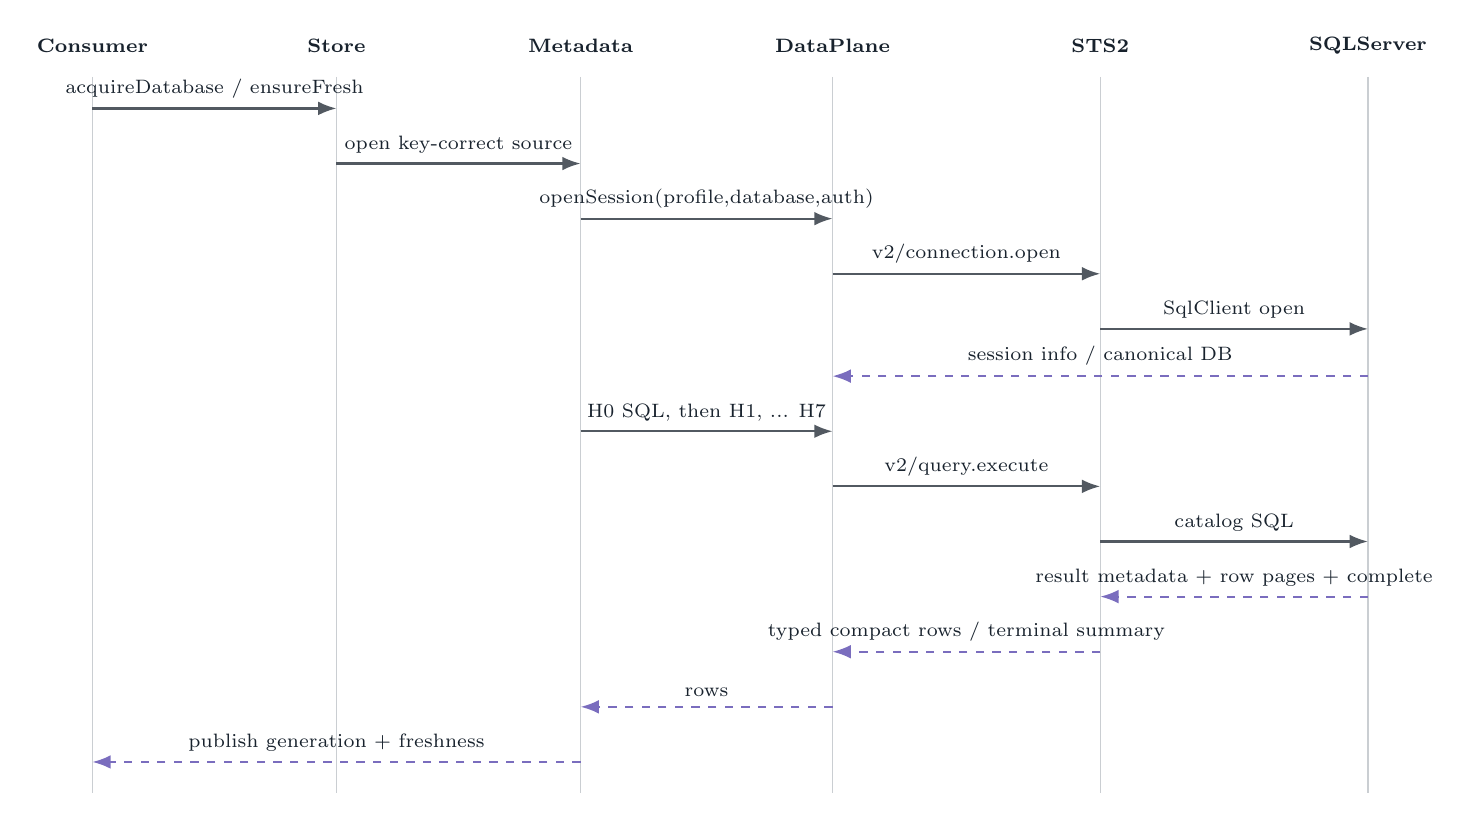
\begin{tikzpicture}
  \foreach \x/\name in {0/Consumer,3.1/Store,6.2/Metadata,9.4/DataPlane,12.8/STS2,16.2/SQLServer} {
    \node[font=\scriptsize\bfseries] (h\name) at (\x,0) {\name};
    \draw[slate!30] (\x,-0.4) -- (\x,-9.5);
  }
  \tikzset{msg/.style={->,thick,draw=ink!75},ret/.style={->,thick,dashed,draw=violetdark!75}}
  \draw[msg] (0,-0.8)--node[above,font=\scriptsize]{acquireDatabase / ensureFresh} (3.1,-0.8);
  \draw[msg] (3.1,-1.5)--node[above,font=\scriptsize]{open key-correct source} (6.2,-1.5);
  \draw[msg] (6.2,-2.2)--node[above,font=\scriptsize]{openSession(profile,database,auth)} (9.4,-2.2);
  \draw[msg] (9.4,-2.9)--node[above,font=\scriptsize]{v2/connection.open} (12.8,-2.9);
  \draw[msg] (12.8,-3.6)--node[above,font=\scriptsize]{SqlClient open} (16.2,-3.6);
  \draw[ret] (16.2,-4.2)--node[above,font=\scriptsize]{session info / canonical DB} (9.4,-4.2);
  \draw[msg] (6.2,-4.9)--node[above,font=\scriptsize]{H0 SQL, then H1, ... H7} (9.4,-4.9);
  \draw[msg] (9.4,-5.6)--node[above,font=\scriptsize]{v2/query.execute} (12.8,-5.6);
  \draw[msg] (12.8,-6.3)--node[above,font=\scriptsize]{catalog SQL} (16.2,-6.3);
  \draw[ret] (16.2,-7.0)--node[above,font=\scriptsize]{result metadata + row pages + complete} (12.8,-7.0);
  \draw[ret] (12.8,-7.7)--node[above,font=\scriptsize]{typed compact rows / terminal summary} (9.4,-7.7);
  \draw[ret] (9.4,-8.4)--node[above,font=\scriptsize]{rows} (6.2,-8.4);
  \draw[ret] (6.2,-9.1)--node[above,font=\scriptsize]{publish generation + freshness} (0,-9.1);
\end{tikzpicture}}
\caption{Current end-to-end path. The metadata service is a catalog-aware client over generic STS2 query execution, not a server-side metadata RPC.}
\label{fig:stssequence}
\end{figure}

\subsection{Why dedicated sessions are the right bridge}

STS2 permits one active query per connection and enforces page-window backpressure and exactly one terminal completion. The database engine correctly serializes its H-ladder, digest, and lazy module work on one session. User query sessions remain independent, so main-lane catalog work does not race with F5 execution.

The auxiliary boundary is only partially complete: server/database auxiliary catalogs have separate sources from the main lane, but different auxiliary section keys can overlap through the same source's cached session. The executable STS2 scenario \path{second-query-while-active-busy.yaml} expects the second execute to fail with \code{Sts2.Busy}. A per-catalog FIFO lane is therefore part of the adapter contract, not optional optimization.

\subsection{One owner for serverless wake and retry}

The SQL Data Plane has two public entry shapes: top-level \code{SqlDataPlaneService.openSession()} and a service view returned by \code{service()} or \code{serviceForProfile()}. The current top-level method obtains the public view and wraps \code{view.openSession()} in \code{openWithServerlessWake()}; the view's \code{openSession()} also wraps the raw provider call in the same helper. The resulting call graph is outer wake $\rightarrow$ inner wake $\rightarrow$ backend open.

Nested wake policy can multiply ARM status checks, delay windows, and open attempts, and makes attribution ambiguous. Choose one owner. The simplest option is for the public view to own requirements, provider availability, session registration, and wake, while the top-level method delegates directly after its pure capability/fallback decision. A spy-based unit test should assert one wake invocation and the exact backend open-attempt count for paused, resuming, and ordinary profiles.

\begin{reviewbox}[title={Related open SQL Data Plane thread}]
A current Copilot thread also notes that a failed provider \code{canOpen()} result is routed through the capability-unsupported error helper, even when the failure represents availability/handshake state. Keep that classification fix separate from the duplicate-wake repair: capability mismatch, backend unavailability, and serverless resume are different error/retry domains.
\end{reviewbox}

\subsection{How dedicated metadata endpoints can fit later}

A future STS2 contract may add endpoints that return server/database sections directly, potentially with server-side paging, digests, or change tokens. The clean migration point is the \code{MetadataSessionSource}/data-source adapter:

\begin{enumerate}
  \item keep \code{CatalogSnapshot}, store keys, lease lifecycle, freshness policies, persistence, and consumer provider unchanged;
  \item add a source that checks \code{metadata.endpoints} and calls the new methods;
  \item retain catalog-SQL fallback only where its declared fidelity is sufficient; and
  \item prove endpoint-vs-SQL provider equivalence with the same snapshot fixtures and invariant suite.
\end{enumerate}

The endpoint should not smuggle consumer policy into STS2. The server can own efficient catalog acquisition and stable wire shapes; the extension should continue to own cross-consumer leases, local persistence policy, VS Code focus/offline behavior, and language/UX degradation.

\section{Logging, diagnostics, and privacy}

\subsection{Extension-side event vocabulary}

The feature emits through the unified \code{diag} core, where every field is classified before reaching live-tail, session storage, perftest, or self-test sinks. Principal event families are:

\begin{table}[H]
\centering
\small
\caption{Metadata observability surface at the extension layer.}
\label{tab:events}
\begin{tabularx}{\textwidth}{@{}p{0.24\textwidth}p{0.29\textwidth}X@{}}
\toprule
\textbf{Family} & \textbf{Representative events} & \textbf{Safe diagnostic meaning}\\
\midrule
Engine & \code{metadata.hydrate}, \code{metadata.ensureFresh}, and validation/drift events & Duration, generation, policy mode/reason, freshness/source, wait, error class; database fields are classified paths.\\
Store & acquire server/database, dispose lease, server/aux hydration, access drift, key-correctness tripwires & Short fingerprint, key kind, cache hit/miss, refcount, generation/readiness/counts; no catalog item names.\\
Cache & \code{load}, \code{save}, \code{hit}, \code{miss}, \code{corrupt}, \code{evict}, \code{clear}, and \code{raceLost} & Fingerprint/hash prefixes, byte/duration counts, fixed age buckets, safe enums, policy-intersection boolean.\\
Performance & \path{mssql.metadata.cache.warmAcquire.begin} / \path{mssql.metadata.cache.warmAcquire.end} & Same-process monotonic marker pair; object count and wait time; feature bucket \code{metadata}.\\
\bottomrule
\end{tabularx}
\end{table}

The generated observability registry is the source of truth, mirrored into the embedded perftest package. Conformance tests check that source-emitted names are registered and marker pairs agree. \code{Perf.featureFor()} maps \code{metadata.*}, \code{metadataStore.*}, \code{metadataCache.*}, and \code{mssql.metadata.*} to the metadata feature.

\subsection{Allowlist and forbidden fields}

Allowed event attributes include short non-reversible fingerprint/hash prefixes, generations, readiness summaries, fixed stale-age buckets, byte/duration/wait counts, safe enum results/reasons/tiers, booleans, and error classes. Forbidden fields include raw object/database names unless classified and redacted at the common choke point, SQL text, result rows, endpoints, connection strings, secrets/tokens, prompt text, module definitions, description values, and content-hash prefixes pending policy review.

The key-correctness tripwires intentionally classify expected/actual database values as \code{source.path}; they do not bypass the central redactor. These events prove that a mismatch was detected, not that publication was prevented. Cache status/clear UI may display local database names to the user, but those names do not become telemetry.

\subsection{Extension diagnostics versus STS2 envelopes}

These are complementary layers:

\begin{itemize}
  \item \textbf{Extension diagnostics} explain consumer/store/cache decisions: why a snapshot was served, rejected, refreshed, or evicted.
  \item \textbf{STS2 envelopes} explain transport/runtime causality: RPC input, reducer output, effects, query pages, terminal events, configuration changes, and runtime health.
\end{itemize}

STS2 journals each sanitized envelope before dispatch, then publishes it in sequence order to best-effort metrics/live-tail/custom sinks. Product capture replaces SQL text and row cells with digest wrappers; secret material lives only in an in-memory side table behind opaque references. The envelope carries run ID, gapless sequence, UTC timestamp, kind/type, session/correlation, causal sequence, config version, payload digest, optional payload, and redaction metadata.

\begin{figure}[H]
\centering
\resizebox{0.98\textwidth}{!}{%
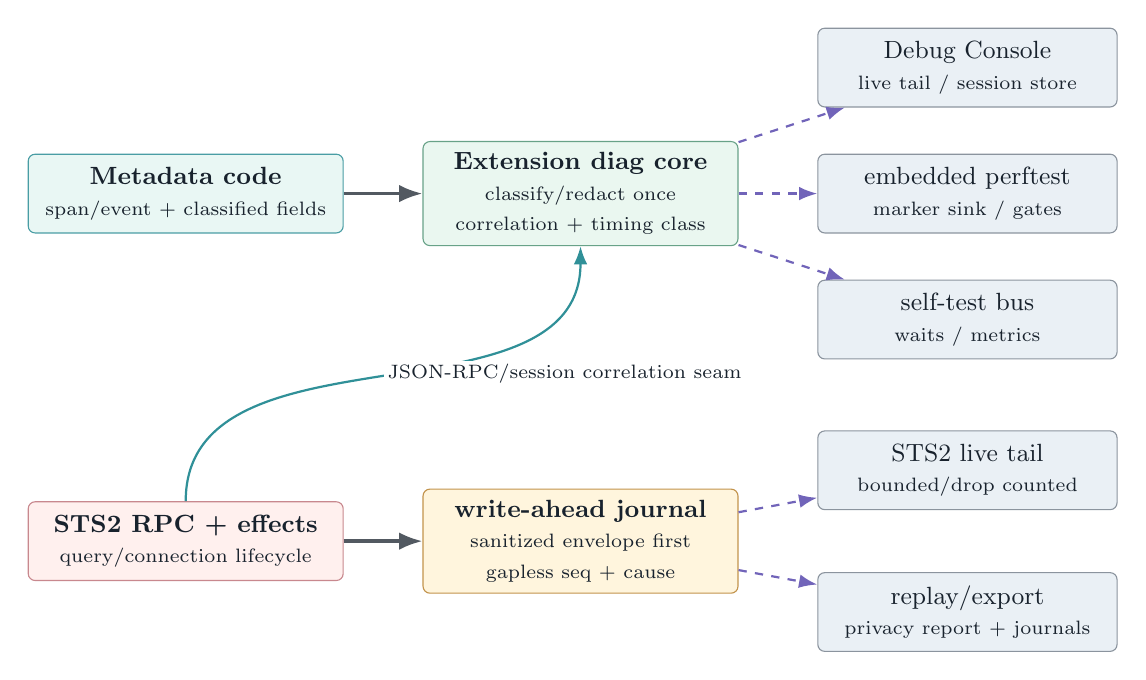
\begin{tikzpicture}[node distance=7mm and 10mm]
  \node[model,minimum width=40mm] (meta) {\textbf{Metadata code}\\\scriptsize span/event + classified fields};
  \node[gate,minimum width=40mm,right=of meta] (diag) {\textbf{Extension diag core}\\\scriptsize classify/redact once\\\scriptsize correlation + timing class};
  \node[comp,minimum width=38mm,right=of diag,yshift=16mm] (live) {Debug Console\\\scriptsize live tail / session store};
  \node[comp,minimum width=38mm,right=of diag] (perf) {embedded perftest\\\scriptsize marker sink / gates};
  \node[comp,minimum width=38mm,right=of diag,yshift=-16mm] (self) {self-test bus\\\scriptsize waits / metrics};

  \node[sess,minimum width=40mm,below=34mm of meta] (rpc) {\textbf{STS2 RPC + effects}\\\scriptsize query/connection lifecycle};
  \node[cache,minimum width=40mm,right=of rpc] (journal) {\textbf{write-ahead journal}\\\scriptsize sanitized envelope first\\\scriptsize gapless seq + cause};
  \node[comp,minimum width=38mm,right=of journal,yshift=9mm] (tail) {STS2 live tail\\\scriptsize bounded/drop counted};
  \node[comp,minimum width=38mm,right=of journal,yshift=-9mm] (bundle) {replay/export\\\scriptsize privacy report + journals};

  \draw[arrow] (meta)--(diag);
  \draw[async] (diag)--(live); \draw[async] (diag)--(perf); \draw[async] (diag)--(self);
  \draw[arrow] (rpc)--(journal);
  \draw[async] (journal)--(tail); \draw[async] (journal)--(bundle);
  \draw[dataarr] (rpc.north) to[out=90,in=-90] node[labelbox,right]{JSON-RPC/session correlation seam} (diag.south);
\end{tikzpicture}}
\caption{Two observability planes. Extension events explain metadata policy; STS2 envelopes explain transport causality. Both are bounded and privacy-classified, and can be stitched without copying SQL or rows into product telemetry.}
\label{fig:observability}
\end{figure}

\section{Test design and coverage}

\subsection{Strength of the current test strategy}

The focused suite is unusually good at semantic failure modes: immutable publication, section readiness, deterministic ordering, exact catalog detail, same-key acquisition, lifecycle disposal, codec bounds, malformed payloads, torn writes, privacy canaries, poll governance, and large-catalog scaling. Prior review comments also drove concrete fixes for quadratic projection, delimiter collisions, UDT rendering, hidden columns, role-owned schemas, untrusted FKs, decompression bounds, content-addressed payloads, and shutdown flush.

The original review found that test volume was high but several unsafe branches were not selected. The repaired head adds those adversarial boundaries directly, so the closure claim rests on exact interleavings and call-count assertions rather than nearby happy paths.

\subsection{Current focused suite inventory}

The correctness-closeout run at \code{e5952174a} reported 158 passing tests across the metadata/cache/catalog files below, including the new auxiliary-catalog suite; adding touched profile-identity, private-preview/manifest, and SQL Data Plane files yielded 206. After merging current \code{main} and adding activation-snapshot coverage, the combined \code{Metadata|AuxiliaryCatalog|SQL Data Plane|PreviewFeaturesService|Private preview manifest|Extension API Tests} selection passed 260/260 at \code{37bf23fce}. The final public-view alternatives fix then passed its owning backend-registry suite 17/17 at \code{69ca292f8}. These are executed-inventory counts, not a claim that every assertion in pre-existing touched files was introduced by this PR.

\begin{longtable}{@{}p{0.25\textwidth}p{0.12\textwidth}p{0.56\textwidth}@{}}
\caption{Metadata closure inventory introduced by \code{e5952174a} and re-executed within the merged-head selection.}\label{tab:testinventory}\\
\toprule
\textbf{Suite} & \textbf{CI count} & \textbf{Principal invariants}\\
\midrule
\endfirsthead
\toprule
\textbf{Suite} & \textbf{CI count} & \textbf{Principal invariants}\\
\midrule
\endhead
\code{metadataCatalog} & 36 & H-ladder parsing, readiness/partial failures, resolution/search, exact-only unknown-case behavior, DDL keyword detection, descriptions, lazy definitions, burst coalescing, hidden columns, safe IDs.\\
\code{metadataCatalogDetail} & 6 & Exact column/FK facts, UDT spelling/schema, identity text, defaults/computed detail, FK actions, and column identity.\\
\code{metadataDeterminism} & 6 & Ordinal ordering, byte-stable schema context, catalog-collation case behavior, and digest-v2 rename detection.\\
\code{metadataFreshness} & 10 & Four policy modes, TTL, timeout-as-race, abort-listener balance, server watchdog/recycle recovery, section gates, and stale/live/unavailable honesty.\\
\code{metadataPoll}\allowbreak\code{Governance} & 12 & Backoff, jitter bounds, focus suspension/resume, serverless cap, limiter behavior, and failure retry.\\
\code{metadataStore} & 13 & A/B key isolation, same-key single flight, routed sessions, leases, refcounts, idle TTL/LRU, cleanup, and server catalogs.\\
\code{metadataStoreCache} & 6 & Disk-before-live publication, manifest generation/digest baseline, background refresh, offline seeded hit, recovery, and A/B isolation with cache.\\
\code{metadataStoreScale} & 6 & 10k-object hydration/counts, ordering/search, 1k-column table, bounded schema context, and warm reacquire without rehydration.\\
\code{metadataStoreService} & 3 & Default-off composition, enabled coordinator, and data-plane-disabled fail-fast without backend acquisition.\\
\code{metadataCacheCodec} & 20 & Live/disk round-trip equivalence, byte stability, content-hash perturbation, privacy stripping, strict shape/range/ownership validation, and model/version misses.\\
\code{metadataCacheStore} & 39 & Path containment, requested-key and logical-hash integrity, oversize bounds, quarantine, rename retry, torn writes, older-last and manifest-only/full writer races, eligibility/skips, policy intersection, privacy canaries, index/eviction/clear/settings.\\
\code{auxiliaryCatalog} & 1 & Two distinct sections started together complete FIFO through one one-active-query session.\\
\midrule
\textbf{Metadata subtotal} & \textbf{158} & Repaired-head local hosted counts; zero failures.\\
\bottomrule
\end{longtable}

This inventory now includes the stronger boundary proofs. The regression matrix below records how each prior finding was closed and remains the checklist to retain through future refactors.

\begin{table}[H]
\centering
\small
\caption{Regression matrix closing the review findings at final head \code{69ca292f8}.}
\label{tab:regressions}
\begin{tabularx}{\textwidth}{@{}p{0.08\textwidth}p{0.28\textwidth}p{0.29\textwidth}X@{}}
\toprule
\textbf{ID} & \textbf{Invariant} & \textbf{Prior gap} & \textbf{Repaired-head proof}\\
\midrule
F1 & Offline setting means zero live work & Seeded hit with polling disabled & Hit, miss, refresh, strict policies, auxiliary, polling, and online$\rightarrow$offline assert resolver/session/query counts remain zero.\\
F2 & Wrong database never publishes; drift/timeout reopens & Correct routing and later digest drift & H0 returns \code{WrongDb}; no snapshot publishes, violation latches, and retry opens a fresh session through forwarded \code{recycle()}.\\
F3 & One active query per auxiliary session & Same-section single flight & Two distinct delayed sections start together; both become ready through one fake one-active-query session.\\
F4 & Cache entry belongs to requested key & Path derivation/containment & A valid A manifest/payload copied into B's directory returns \code{keyMismatch} and is invalidated.\\
F5 & Newer authority cannot be overwritten & Post-save winner observation & Per-key lock tests force older-last and delayed manifest-only/full interleavings; capture time beats local generation and new data remains authoritative.\\
F6 & One serverless wake policy per open & Registry/view tripwires & Top-level open reaches the provider exactly once; the existing eight-case wake suite pins eligible retry bounds; provider refusal is retryable unavailable.\\
F7 & Wait abort listener is removed & Server service only & Database service proves add/remove balance after success and timeout while reusing the same signal.\\
F8 & Unknown case rule never folds optimistically & H0 success and collation divergence & Unknown semantics resolve exact spellings independently and reject a folded-only spelling.\\
F9 & Server refresh recovers from hung completion & Caller timeout race & Swallowed server completion times out, publishes failed/not-empty truth, recycles, and succeeds on the next refresh; epoch fencing blocks late mutation.\\
F10 & Manifest logical hash matches decoded payload & SHA and canonical hash separately & Valid compressed SHA and payload shape with a false \code{contentHash} returns corrupt and quarantines.\\
\bottomrule
\end{tabularx}
\end{table}

\subsection{Persistence tests remain protocol tests}

Cache tests should continue to model filesystem operations as a protocol, not as ordinary serialization coverage. The completed suite already covers many crash points and corruption classes. The next additions must distinguish three layers:

\begin{itemize}
  \item \textbf{byte safety}: size, SHA, gzip bound, JSON and array invariants;
  \item \textbf{identity safety}: requested key and logical content hash;
  \item \textbf{authority safety}: one atomic, globally comparable publication decision per key.
\end{itemize}

A result such as \code{raceLost} is only meaningful if the final manifest is known to represent the winning authority. Post-save writer-ID comparison alone does not prove that when an older writer installs last.

\subsection{Embedded perftest coverage}

The embedded scenario \code{metadatacache-warm-acquire} is the correct performance boundary: cold fill/save, a fresh store in offline mode, disk verification and rehydration/publication, source-honesty assertion, and begin/end markers around only the warm acquire. It is exploratory rather than an official SLA gate. Before graduation it should run across representative catalog sizes, Windows/macOS/Linux, local and remote extension hosts, and repeated cold/warm profiles with pre-registered p50/p95 budgets.

The repaired offline unit matrix asserts resolver calls and session opens directly rather than relying only on a \code{disk} source label. The embedded performance scenario should retain the same counters if promoted from exploratory measurement to an SLA gate.

Local package verification in this work session built the embedded perftest workspace and ran 347 tests passing with 16 explicit skips. Fifteen skips are central-store integrations and one is vendor-sync; the Query Studio scenario tests (158) and VS Code spawn tests (2) passed. This verifies registry/contracts/harness behavior, not a live SQL warm-cache benchmark run against a provisioned \code{PerfHarness} database.

\subsection{Coverage evidence and its limit}

Codecov at the pinned head reports 91.09384\% patch coverage with 894 changed lines uncovered. Project coverage rises from 77.17\% at the PR base to 77.96\% at the head. Core metadata files are strong---catalog model 97.22\%, codec 95.81\%, coordinator 96.20\%, store 94.47\%, and engine 93.44\%---while host wiring and broad auxiliary surfaces are weaker: main controller 9.38\%, database auxiliary sections 73.75\%, auxiliary engine 77.44\%, and store composition service 86.53\%.

Coverage supports the focused suites but does not settle the review findings. Race ordering, dynamic network authorization, key binding, and retry ownership are semantic properties; they require the deterministic adversarial tests in \cref{tab:regressions}, not merely more executed lines.

\section{Build and validation record}

\subsection{Current GitHub state observed independently}

At prior head \code{9955ff9e6}, analysis/CodeQL, Azure PR validation, packaging, normalization, CLA, and all six platform VSIX-launch jobs passed. Its GitHub \code{build-and-test} check was red, but its metadata-relevant facts were more specific:

\begin{itemize}
  \item extension install/build, lint, package, and MSSQL unit-test steps pass;
  \item the GitHub unit runner reports 3,975 passing, 0 failing, and 12 skipped;
  \item every metadata file in \cref{tab:testinventory} reports zero failures;
  \item the aggregate job fails because SQL Projects unit tests return exit code 1 and one of 17 VSIX smoke tests---``MSSQL add connection webview is loaded correctly''---fails.
\end{itemize}

This was not evidence of a metadata failure. The later correctness head became conflicting as \code{main} advanced. Merge commit \code{37bf23fce} incorporates current \code{main} and resolves that conflict; its build/test workflow passed. Five of six platform launch jobs also passed. The sole win-x64 failure occurred in test-dependency installation: \code{npm ci} reported Windows \code{EPERM} cleanup failures under \code{monaco-editor}, then git-dependency preparation exited nonzero. Artifact download and the extension-launch step were skipped, so that red workflow contains no product-runtime failure. Final head \code{69ca292f8} adds only the reviewed public-view alternatives repair. At the final delayed-review snapshot, both analysis jobs, aggregate CodeQL, normalization, CLA, and MSSQL VSIX packaging were green. Aggregate build/test and all six platform VSIX-launch jobs remained in progress; live PR checks remain the authority for the eventual merge button.

\subsection{Independent local validation}

The local workspace was updated and built at the pinned commits before this report. Results are kept separate from PR-author comments and GitHub CI:

\begin{table}[H]
\centering
\small
\caption{Independent local validation snapshot, updated 29 August 2026.}
\label{tab:localvalidation}
\begin{tabularx}{\textwidth}{@{}p{0.25\textwidth}p{0.26\textwidth}X@{}}
\toprule
\textbf{Lane} & \textbf{Result} & \textbf{Interpretation / explicit exclusions}\\
\midrule
vscode-mssql build & Pass & Full monorepo build repeated on \code{69ca292f8}: shared toolkit, MSSQL extension/typecheck/bundles/webviews/notebook renderer, merged SQL Projects runtime, legacy SQL Database Projects package, and Data Workspace.\\
vscode-mssql lint & Pass & Root lint exited zero for extension-toolkit, MSSQL, SQL Database Projects, and Data Workspace.\\
Focused tests & 260 pass; 0 fail at \code{37bf23fce}; 17 pass; 0 fail at \code{69ca292f8} & Broad metadata/cache/catalog, auxiliary, profile/preview/manifest, SQL Data Plane, and activation-context selection followed by the owning backend-registry suite for the final alternatives fix.\\
MSSQL broad hosted tests & 4,025 pass; 0 fail; 10 skip at merge parent \code{37bf23fce} & Complete inverse selection excludes exactly \code{QueryCompletionSoundService} and \code{Utility Tests - Path handling}. The full run otherwise reports eight failures, all reproduced alone as untouched Windows path-separator expectations (seven sound, one tilde path). The final change is restricted to returning already-computed alternative identifiers and its focused suite, full build, and full lint were rerun.\\
SQL Projects hosted tests & 205 pass; 0 fail; 6 skip & Current-main isolated SQL Database Projects unit lane, run in a separate VS Code host as required by the merged test configuration.\\
Localization & Pass & Root extraction processed all four projects and extracted 3,064 MSSQL strings; commit hooks repeated extraction and lint-staged successfully.\\
Direct packaging & Pass & MSSQL produced 2,453 files / 208.53 MiB with the worktree's existing 617.8 MiB expanded STS payload. SQL Projects produced 428.41 KiB, Data Workspace 17.10 KiB, and the keymap 7.14 KiB. The root wrapper cannot forward MSSQL-only \code{--online --skip-service-install} through SQL Projects because \code{vsce} rejects \code{--online}; direct workspace packages prove the artifacts themselves.\\
Embedded perftest & 347 pass; 16 skip & All package tests/builds pass; skips are described above; the live provisioned warm-cache scenario was not executed.\\
sqltoolsservice Release solution & Pass; serial MSBuild with shared compilation disabled & 0 errors; two ScriptDom locale warnings.\\
STS2 unit + E2E & 496 pass / 10 SQL-server-gated skip; 6/6 E2E & Deterministic/runtime contract and process interop green; engine-gated skips explicitly reported.\\
STS auth / language & 9/9; 76/76 & Adjacent authentication and current language-service lanes green.\\
ServiceLayer unit & 1,944 pass; 1 fail & One platform/provider DNS failure, not metadata logic. No on-prem integration lane was provisioned.\\
\bottomrule
\end{tabularx}
\end{table}

\begin{evidencebox}
The local runs establish that the repaired tree builds/packages and close F1--F10 with deterministic unit regressions. They do not replace live SQL compatibility testing, the provisioned warm-cache scenario, or on-prem/remote-host performance matrices; those remain graduation gates rather than merge blockers for this default-off substrate.
\end{evidencebox}

\subsection{Author- and review-reported evidence}

The PR body reports additional focused host-composition, data-plane capability, observability, localization, packaging, and full-suite results. Prior review threads report targeted performance probes and repeated focused suites after earlier fixes. These are useful confidence signals and should remain in the PR record, but they are \reported{} rather than rerun as part of this review pass.

All 52 review threads are resolved at the pinned head with source-attributed dispositions. Provider startup refusal is retryable \code{unavailable}; the QuickPick separates localized capture text from fingerprint detail; activation-snapshot keys prevent pre-reload command exposure; and bound service views retain registry alternatives on a requirement failure. The CR-only line-comment suggestion was declined at the raised closeout threshold: VS Code documents support LF/CRLF, both are handled, and a synthetic CR-only miss would merely defer the best-effort DDL refresh to digest polling.

\section{Performance mechanisms and evidence quality}

The implementation removes the most important algorithmic traps:

\begin{itemize}
  \item constant-time object-ID lookup during build;
  \item value-by-value row-page append rather than spreading unbounded arguments;
  \item snapshot indexes for name/prefix lookup;
  \item linear schema-context candidate rendering per fidelity tier;
  \item same-key acquisition, validation, and forced-refresh coalescing;
  \item content-equal cache saves reduced to a manifest update;
  \item delayed/throttled maintenance outside activation;
  \item focus-gated, backoff/jittered, per-server-limited polling.
\end{itemize}

Prior review measurements show that the fixed scale paths are orders of magnitude better than the earlier quadratic implementation. Those measurements are review-machine observations, not product SLAs. The repaired single wake owner and auxiliary FIFO remove the two policy-multiplication risks identified in the prior review; lock contention and cache-load latency should still be measured across local/remote filesystems before enabling persistence by default.

A graduation performance plan should separate:

\begin{enumerate}
  \item live H0--H7 hydration CPU, SQL time, memory peak, and payload size;
  \item warm cache read, hash/decompress/validate, and publication time;
  \item interactive snapshot query/projection latency with no network;
  \item background poll/validation cost under focus, resume storms, and serverless pause; and
  \item multi-window contention/lock hold time after the authority fix.
\end{enumerate}

\section{Mechanism-to-evidence traceability}

\begin{table}[H]
\centering
\small
\caption{Load-bearing mechanisms and repaired-head closure evidence.}
\label{tab:traceability}
\begin{tabularx}{\textwidth}{@{}p{0.24\textwidth}p{0.32\textwidth}X@{}}
\toprule
\textbf{Mechanism} & \textbf{Current evidence} & \textbf{Disposition}\\
\midrule
Same-key single flight & Eight-way concurrency tests and explicit disposal coverage & Retain.\\
Immutable deterministic snapshot & Catalog/detail/determinism/round-trip/scale plus unknown-case exact-only regression & Closed; retain.\\
Database identity & H0 mismatch-before-publication, violation latch, recycle/reopen and disposal-race tests & Closed; live SQL collation/database corpus remains a graduation gate.\\
Offline behavior & Dynamic resolver/engine/server/auxiliary gate with hit/miss/transition call-count matrix & Closed.\\
STS2 one-query discipline & Main lane, catalog-wide auxiliary FIFO, database/server watchdog and recycle tests & Closed.\\
Cache byte integrity & Content addressing, SHA/gzip/shape, requested-key copy test, canonical logical-hash test & Closed.\\
Cache cross-window authority & Per-key lock, capture-time ordering, older-last and manifest-only/full interleaves & Closed for catalog authority; advisory index LRU remains documented approximate.\\
Privacy at rest & Codec stripping, manifest policy, disk canaries rerun after cache changes & Closed; retain.\\
Data-plane capability/auth & Pure tripwires, retryable availability classification, one top-level provider open, wake suite & Closed.\\
Consumer seam & Lease/snapshot/freshness APIs and refactor designs & Future provider equivalence, pinned-generation, no-keystroke-I/O, and honesty corpus.\\
\bottomrule
\end{tabularx}
\end{table}

\section{Known boundaries and next validation gates}

\subsection{Model enrichments deliberately deferred}

The substrate reports rather than conceals incomplete domains. Synonym target traversal, table-type shapes, sequences, parameter/schema descriptions, row counts, and section/object-level T2/T3 digests need new model/API shapes. They should land with consumers that can exercise them end to end, not as unreachable arrays that misleadingly say \code{ready}.

\subsection{Integration work for the native language service}

The following gates should precede a language cutover:

\begin{enumerate}
  \item retain the now-closed F1--F3 regressions so offline, identity, and STS2 lane contracts remain trustworthy;
  \item implement the provider adapter and prove fixture/null/catalog provider equivalence;
  \item pin one generation per feature request and test a mid-request generation change;
  \item prove completion/hover/diagnostics make no network call on the keystroke path;
  \item run the honesty corpus: temp tables, CTEs, dynamic SQL, synonyms, cross-database names, case-sensitive catalogs, partial/offline metadata, and \code{USE} changes;
  \item define suppression/status UX for unavailable sections and stale/offline snapshots;
  \item benchmark real completion p50/p95 and document CPU/memory budgets separately from cache load.
\end{enumerate}

\subsection{Integration work for dedicated STS2 endpoints}

Before flipping \code{metadata.endpoints} to supported:

\begin{enumerate}
  \item add generated wire-contract methods and stable error shapes in STS2;
  \item define section/readiness semantics and paging/backpressure for large catalogs;
  \item preserve database-key correctness and one-terminal cleanup under cancel/dispose;
  \item decide whether STS2 returns canonical arrays, row-like sections, or a provider-neutral DTO---without importing the extension cache format as wire format;
  \item produce a live-SQL truth corpus and endpoint-vs-catalog-SQL snapshot-equivalence tests;
  \item extend STS2 envelope/privacy canaries so metadata names and definitions follow explicit capture policy.
\end{enumerate}

\subsection{Completed closeout plan}\label{sec:blockers}

\begin{table}[H]
\centering
\small
\caption{Completed repair and merge-closeout order for PR \#22836 at \code{69ca292f8}.}
\label{tab:repairorder}
\begin{tabularx}{\textwidth}{@{}p{0.08\textwidth}p{0.30\textwidth}X@{}}
\toprule
\textbf{Order} & \textbf{Repair} & \textbf{Closure status}\\
\midrule
1 & F2 fail-closed identity + recycle forwarding & Implemented; mismatch cannot publish and later retry reopens.\\
2 & F1 dynamic offline network gate & Implemented across store, engines, timers, definitions, and auxiliary paths.\\
3 & F3 auxiliary FIFO + F9 server watchdog & Implemented and regression-tested.\\
4 & F4 key binding + F10 logical-hash verification & Implemented and corruption/copy-tested.\\
5 & F5 per-key cross-window authority & Implemented with exclusive-create lock and adversarial interleavings.\\
6 & F6 single wake owner + availability classification & Implemented; registry/conformance/wake suites pass.\\
7 & F7 abort listener + F8 unknown case behavior + index documentation & Implemented; advisory cross-window LRU explicitly accepted as approximate.\\
8 & Full focused suites, broad hosted suite, build/lint/package, Actions rerun & Local gates complete; fresh GitHub Actions triggered. Live SQL/performance matrices remain pre-graduation work.\\
\bottomrule
\end{tabularx}
\end{table}

\section{Final assessment}

\begin{takeawaybox}
The architectural direction is good: one shared lease/store, immutable compact snapshots, explicit per-section truth, policy-routed freshness, default-off persistence, content-addressed payloads, and a future transport/provider seam are the right foundations for native language and AI-assisted SQL experiences.

At \code{69ca292f8}, the implementation enforces the design narrative's load-bearing claims: zero-network offline operation, key-correct publication, one-active-query auxiliary behavior, newer-writer cache authority, decoded logical integrity, bounded hydration recovery, one serverless wake owner, activation-consistent preview UI, and capability-alternative parity across public data-plane views. The feature remains private-preview/default-off and no ordinary language, AI, OE, or Query Studio surface is cut over by this PR.
\end{takeawaybox}

\begin{statusbox}[title={Decision statement}]
Recommended disposition: code/design review findings are closed; proceed to CI and human merge review. Do not enable the substrate by default or cut over consumers based only on these unit/build results. Live SQL compatibility, remote-host cache behavior, and real workload performance remain graduation gates for later preview stages.
\end{statusbox}

\section*{Evidence and source map}
\addcontentsline{toc}{section}{Evidence and source map}

\normalsize
\begin{statusbox}[title={Reproducibility note}]
This report is pinned because the PR and related branches are active. Review threads, Actions conclusions, and code locations are observations at the stated snapshot, not timeless properties. Re-fetch the head, rerun the specified regression and whole-PR lanes, and update the title-page pins and disposition before using the PDF after any new commit.
\end{statusbox}

\small
\begin{longtable}{@{}>{\raggedright\arraybackslash}p{0.23\textwidth}>{\raggedright\arraybackslash}p{0.70\textwidth}@{}}
\toprule
\textbf{Evidence class} & \textbf{Primary sources used}\\
\midrule
PR state & \href{https://github.com/microsoft/vscode-mssql/pull/22836}{PR \#22836}, current body/discussions/check metadata, merge-ready head \code{69ca292f8}, current-main merge \code{37bf23fce}, main parent \code{59c8ea50c}, extraction base \code{69f54be2a}.\\
Core implementation & \path{extensions/mssql/src/services/metadata/catalogModel.ts}; \path{metadataService.ts}; \path{metadataStore.ts}; \path{metadataStoreService.ts}; \path{serverMetadataService.ts}; \path{auxiliaryCatalog*.ts}; profile/auth/fingerprint modules.\\
Cache implementation & \path{extensions/mssql/src/services/metadata/cache/metadataCacheCodec.ts}; \path{metadataCacheManifest.ts}; \path{metadataCacheStore.ts}; \path{metadataCacheCoordinator.ts}; \path{metadataFreshness.ts}; \path{metadataCacheSettings.ts}.\\
Host/data plane & \path{mainController.ts}; \path{previewService.ts}; \path{sqlDataPlaneService.ts}; \path{languageservice/serviceclient.ts}; package settings/localization; \path{perfTelemetry.ts}.\\
Tests & Metadata/cache/catalog/freshness/poll/store/scale suites, profile and data-plane tests, observability conformance, large-catalog fixture, and in-memory filesystem harness; CI per-file counts plus the independent local validation in \cref{tab:localvalidation}.\\
Embedded perftest & \path{tools/perftest/packages/perftest-cli/src/scenarios/registry.ts} and the metadata warm-acquire command/marker wiring.\\
Implementation review & Companion workspace review \path{vscode_mssql_pr_22836_code_review.md}; every finding was rechecked against local and pushed head \code{69ca292f8} before publication.\\
Metadata/refactor designs & \path{vscode-ext-refactor/metadata-docs/*}, including substrate, cache/drift, and review addendum documents; current code controls when design notes and implementation differ.\\
Language/observability designs & Native T-SQL language-service and observability notes under \path{vscode-ext-refactor}; treated as downstream contracts, not PR content.\\
STS2 authority & \code{microsoft/sqltoolsservice dev/query} at \code{fe8300939}: generated contract, \path{docs/sts2/INVARIANTS.md}, runtime/client documentation, and \path{test/sts2/scenarios/second-query-while-active-busy.yaml}.\\
\bottomrule
\end{longtable}


\end{document}
